%\documentclass[10pt]{article}
\documentclass[10pt]{book}
\def\baselinestretch{1.1}
\usepackage[bookmarks]{hyperref}
\usepackage{kotex} % korean tex
\usepackage[utf8]{inputenc} % set input encoding (not needed with XeLaTeX)
\usepackage{framed}
\usepackage{geometry} % to change the page dimensions
\geometry{letterpaper} % or letterpaper (US) or a5paper or....
% \geometry{margins=2in} % for example, change the margins 
%to 2 inches all round
% \geometry{landscape} % set up the page for landscape
%   read geometry.pdf for detailed page layout information
\usepackage{listings}
\lstset{language=[90]Fortran,
	basicstyle=\ttfamily,
	keywordstyle=\color{red},
	commentstyle=\color{green},
	morecomment=[l]{!\ }% Comment only with space after !
}
% Fortran code example
%\begin{lstlisting}[frame=single]
%! Der folgende Fortran-Code ist bei Wikipedia geklaut.
%SUBROUTINE test( Argument1, Argument2, Argument3 )
%   REAL,              INTENT(IN) :: Argument1
%   CHARACTER(LEN= *), INTENT(IN) :: Argument2
%   INTEGER,           INTENT(IN), OPTIONAL :: Argument3
%   ! This makes sense
%END SUBROUTINE
%\end{lstlisting} 
%-----------------------------
\usepackage{graphicx} % support the \includegraphics command and options

% \usepackage[parfill]{parskip} % Activate to begin paragraphs 
%with an empty line rather than an indent

\usepackage{booktabs} % for much better looking tables
\usepackage{array} % for better arrays (eg matrices) in maths
\usepackage{paralist} % very flexible & customisable lists 
%(eg. enumerate/itemize, etc.)
\usepackage{verbatim} % adds environment for commenting 
% out blocks of text & for better verbatim
\usepackage{subfig} % make it possible to include 
%more than one captioned figure/table in a single float
% These packages are all incorporated in the memoir class 
%to one degree or another...

%%% HEADERS & FOOTERS
\usepackage{fancyhdr} % This should be set 
% AFTER setting up the page geometry
\pagestyle{fancy} % options: empty , plain , fancy
\renewcommand{\headrulewidth}{0pt} % customise the layout...
\lhead{}\chead{}\rhead{}
\lfoot{}\cfoot{\thepage}\rfoot{}

%%% SECTION TITLE APPEARANCE
\usepackage{sectsty}
\allsectionsfont{\sffamily\mdseries\upshape} 
% (See the fntguide.pdf for font help)
% (This matches ConTeXt defaults)

%%% ToC (table of contents) APPEARANCE
\usepackage[nottoc,notlof,notlot]{tocbibind} 
% Put the bibliography in the ToC
\usepackage[titles,subfigure]{tocloft} 
% Alter the style of the Table of Contents
\renewcommand{\cftsecfont}{\rmfamily\mdseries\upshape}
\renewcommand{\cftsecpagefont}{\rmfamily\mdseries\upshape} % No bold!

\usepackage{amsmath}
\usepackage{amssymb}
\usepackage{epsfig}
\usepackage{color}

\usepackage{empheq}
% make possible to box equations, For example
%\begin{empheq}[box=\fbox]{align*}
%a&=b \tag{test}\\
%E&=mc^2 + \int_a^a x\, dx
%\end{empheq}

\parindent 10pt\textheight 9in\topmargin -0.4in\textwidth 6in
\oddsidemargin .25in\evensidemargin 0in
\def\bm{\boldsymbol}
\newcommand{\bea}{\begin{eqnarray}}
\newcommand{\eea}{\end{eqnarray}}
\newcommand{\be}{\begin{eqnarray}}
\newcommand{\ee}{\end{eqnarray}}
\newcommand{\no}{\nonumber \\}
\newcommand{\nnb}{\nonumber}
\newcommand{\etal}{{\it et al.}~}
\newcommand{\eg}{{\it e.g.}}
\newcommand{\ie}{{\it i.e.}}
\newcommand{\sll}[1]{#1\hspace{-0.5em}/}
\newcommand{\del}{\partial}
\def\vs{{\bm \sigma}}

\def\vh{{\bm h}}
\def\vk{{\bm k}}
\def\vl{{\bm l}}
\def\vm{{\bm m}}
\def\vn{{\bm n}}
\def\vp{{\bm p}}
\def\vq{{\bm q}}
\def\vr{{\bm r}}
\def\vR{{\bm R}}
\def\vv{{\bm v}}
\def\vx{{\bm x}}
\def\vy{{\bm y}}

\def\la{\langle}
\def\ra{\rangle}

\newcommand{\colmtwo}[2]
{\left(\begin{tabular}{c} {$#1$}\\{$#2$}\end{tabular}\right)}

\newcommand{\colmthr}[3]
{\left(\begin{tabular}{c} {$#1$}\\{$#2$}\\{$#3$}\end{tabular}\right)}

\newcommand{\twodmat}[4]
{\left(\begin{tabular}{cc} {$#1$}&{$#2$}\\
		{$#3$}&{$#4$}\end{tabular}\right)}
\newcommand{\threedmat}[9]
{\left(\begin{tabular}{ccc} {$#1$}&{$#2$}&{$#3$} \\
		{$#4$}&{$#5$}&{$#6$}\\
		{$#7$}&{$#8$}&{$#9$}\\
	    \end{tabular}\right)}	
\newcommand{\threejsymbol}[6]
{\left(\begin{tabular}{ccc} {$#1$}&{$#2$}&{$#3$}\\
                             {$#4$}&{$#5$}&{$#6$}\end{tabular}\right)}
\newcommand{\sixjsymbol}[6]
{\left\{\begin{tabular}{ccc} {$#1$}&{$#2$}&{$#3$}\\
                             {$#4$}&{$#5$}&{$#6$} \end{tabular}\right\}}


%%% The "real" document content comes below...

\title{Lattice EFT note 3: BCC lattice}
\author{Young-Ho Song}
\date{\today}
%\date{} % Activate to display a given date or no date (if empty),
         % otherwise the current date is printed 

\begin{document}
\maketitle
\tableofcontents
\newpage

\chapter{Introduction}

The object of this note is to develop a formalism of lattice EFT calculation
for non-cubic lattice(BCC or FCC). 
There may be two motivation. (1) To test the dependence(or independence) 
of physical observables on the lattice artifacts(lattice size, shape, etc.)  
(2) To compare the numerical efficiency between different lattice formulation. 
(Other motivation?)



\section{Discrete Fourier Transform on a lattice}
General introduction for DFT.

\subsection{1-d case}
\begin{itemize}
	\item For 1D DFT of size N, a sampling(image) is a function, $a(j)$, defined
	at the points, $j\in[N]$, where a subset $[N]:={0,1,2,\dots N-1} $.
	\item DFT is a mapping
	\bea 
	\hat{a}(k)=\frac{1}{\sqrt{N}}\sum_{j\in[N]} a(j) e^{-2\pi i \frac{jk}{N} }, k\in [N]
	\eea 
	\item If the $a(j)$ are purely real, we have a relation
	\bea 
	\hat{a}(k)=\hat{a}(-k)^*=\hat{a}(N-k)^* . 
	\eea 
	Thus, one can obtain $\hat{a}(k> N/2+1)$ from $\hat{a}(k\leq N/2)$. 
	(Also, $\hat{a}(0)$ and $\hat{a}(N/2)$ are real.)
	\item FFTW use this symmetry for r2c or c2r transformation and thus
	the dimension of input and output is different. Real array
	have dimension $N$ and complex array have dimension $N/2+1$ in r2c or c2r of FFTW.
\end{itemize}

\subsection{2-d and 3-d case}
\begin{itemize}
	\item In a similar way, 2-d DFT of size $N_1\times N_2$ can be written as
	\bea 
	\hat{a}(k_1,k_2)=\frac{1}{\sqrt{N_1 N_2}}\sum_{j_1\in[N_1], j_2\in [N_2]} a(j_1,j_2) e^{-2\pi i \frac{j_1 k_1}{N_1} -2\pi i \frac{j_2 k_2}{N_2}}
	\eea 
	where $k_1 \in [N_1]$ and $k_2\in [N_2]$.
	\item In case of real function values $a$, we get relation
	\bea 
	\hat{a}(k_1,k_2)=\hat{a}^*(-k_1,-k_2)=\hat{a}^*(N-k_1,N-k_2)
	\eea 
	\item In a similar way, 3-d DFT of size $N_1\times N_2\times N_3$ can be written as
	\bea 
	\hat{a}(k_1,k_2,k_3)=\frac{1}{\sqrt{N_1 N_2 N_3}}\sum_{j_1\in[N_1], j_2\in [N_2], j_3\in [N_3]} 
	a(j_1,j_2,j_3) e^{-2\pi i \frac{j_1 k_1}{N_1} -2\pi i \frac{j_2 k_2}{N_2}-2\pi i \frac{j_3 k_3}{N_3}}
	\eea 
	where $k_1 \in [N_1]$, $k_2\in [N_2]$ and $k_3\in [N_3]$.
	\item A similar relation for real function values $a$, we get 
	\bea 
	\hat{a}(k_1,k_2,k_3)=\hat{a}^*(-k_1,-k_2,-k_3)=\hat{a}^*(N-k_1,N-k_2,N-k_3).
	\eea  
\end{itemize}

\section{FFT on lattice}
This is a summary of \cite{Zheng} with additional comments. 

\subsection{d-dimensional lattice}
\begin{itemize}
\item Lattice $L$ is set of points generated by basis vectors,
\bea 
L:=\left\{ \sum_{i=1}^d k_i {\bm u}_i, k_i\in Z\right\}.
\eea 
\item sampling matrix of generator matrix ${\bm U}$ is a matrix with basis vectors as columns. 
\item Sublattice $L_0$ is a d-dimensional lattice which is also a subset of lattice $L$. 
      The generator of sublattice $L_0$ is denoted as ${\bm V}$. 
      A periodicity matrix ${\bm M}$ relates ${\bm V}$ (the generator of sublattice $L_0$)
      with ${\bm U}$(generator of $L$) , ${\bm V}={\bm U}{\bm M}$.  
      The periodicity matrix can be written as ${\bm M}={\bm E}{\bm D}{\bm F}$
      with uni-modular matrix ${\bm E}$, ${\bm F}$ and diagonal matrix ${\bm D}$.
      
\item Quotient group $L/L_0:=\{{\bm x}+L_0 :{\bm x}\in L \}$. 
      the coset ${\bm x}+L_0$ is denoted $\bar{\bm x}$.
     If $S\subset L$ such that $\{\bar{\bm s}: {\bm s}\in S\}=L/L_0$ and $\bar{\bm a}\neq \bar{\bm b}$
     whenever ${\bm a},{\bm b}\neq S$ with ${\bm a}\neq {\bm b}$, 
     ${\bf S}$ is called a set of coset representatives of the quotient group $L/L_0$.
\item dual lattice(reciprocal lattice) of $L$ is 
\bea 
L^* :=\{ {\bm s}\in R^d: \la {\bm r},{\bm s}\ra \in Z \mbox{ for each } {\bm r} \in L   \}
\eea 
where $\la {\bm r},{\bm s}\ra $ denotes the inner product. 

If $L_0$ is a sublattice of $L$ and $L^*$ is a sublattice of $L^*_0$, the two quotient groups
$G=L/L_0$ and $\widehat{G}=L_0^*/ L_0^*$ are congruent. 

\item If ${\bm U}$ is a generator of the lattice $L$, ${\bm U}^{-T}$ is a generator of the dual lattice 
$L^*$. Dual lattice (in frequency space or reciprocal lattice) 
$L^*$($L_0^*$) is generated from 
generator matrix $\tilde{U}$($\tilde{V}$),
\bea 
\tilde{\bm U}=({\color{red}\bm U}^{-1})^T,\quad \tilde{\bm V}=({\color{red} \bm V}^{-1})^T.
\eea 

(short proof) For any lattice point $\vr\in L$, there is 
an integer set $[\vr]$ such that $\vr=U[\vr]$. 
If $\vs$ can be written as ${\bm s}=(U^{-1})^T[\vs]$ with an integer set $[{\bm s}]$,
we can see $\la \vr,{\bm s} \ra=\vr^T \cdot {\bm s}=[\vr]^T\cdot [{\bm s}]=$(integer). 
Thus, the reciprocal lattice can be generated with $(U^{-1})^T$

\item Let quotient groups $G=L/L_0$ in position space and $\hat{G}=L_0^*/L^*$ in frequency. 
Let $P$($\hat{P}$) be a set of coset representatives of the 
quotient group $G$($\hat{G}$). Then for any ${\bm r}\in P$, there exists $[{\bm r}]\in Z^d$ such that
${\bm r}={\bm U}\cdot[{\bm r}]$. Similarly, for any ${\bm s}\in \hat{P}$, there exists
$[{\bm s}]_{\tilde V}\in Z^d$ such that ${\bm s}=\tilde{\bm V}[{\bm s}]_{\tilde V}$.
(In other words, when $\vr$ is a Cartesian coordinates of a lattice point, 
$[\vr]$ is its coordinates in generator basis of the lattice L. Similarly, 
${\bm s}$ is a frequency in Cartesian coordinates and $[{\bm s}]$ in  generator basis of $L^*$.)
Thus, 
\bea 
\la {\bm r},{\bm s}\ra &=&{\bm r}^T\cdot{\bm s}
=({\bm U}\cdot[{\bm r}])^T\cdot\tilde{\bm V}\cdot[{\bm s}]_{\tilde{\bm V}}
=({\bm U}\cdot[{\bm r}])^T\cdot ({\bm V}^{-1})^T\cdot[{\bm s}]_{\tilde{\bm V}} \no 
&=&[{\bm r}]^T\cdot {\bm U}^T ({\bm U}\cdot{\bm M})^{-1,T}
\cdot[{\bm s}]_{\tilde{\bm V}} \no 
&=&[{\bm r}]^T\cdot({\bm M}^{-1})^T \cdot [{\bm s}]_{\tilde V} \no 
&=&\left({\color{red}{\bm E}^{-1}}\cdot[{\bm r}]\right)^T\cdot({\bm D}^{-1})^T 
\cdot \left(({\bm F}^{-1})^T [{\bm s}]_{\tilde V}\right) 
\eea     
   
\end{itemize} 

\subsection{DFT on d-dimensional lattice}
\begin{itemize} 
\item DFT on the quotient group G is the mapping ${\cal F}:a\to \hat{a}$ from $C^G$ to $C^{\hat{G}}$
defined by 
\bea 
\hat{a}(\bar{s})=\frac{1}{\sqrt{|G|}}\sum_{\bar{r}\in G} a(\bar{r})\cdot e^{-2\pi i \la {\bm r},{\bm s}\ra} 
\eea 
for each $\bar{s}:=s+L^*\in \hat{G}$, where ${\bm s}$ is an element in $L_0^*$ such that $s+L^*=\bar{s}$.

\item Inverse FT is
\bea 
a(\bar{r})=\frac{1}{\sqrt{|G|}}\sum_{\bar{s}\in \hat{G}}\hat{a}(\bar{s})\cdot 
e^{2\pi i \la {\bm r},{\bm s}\ra }
\eea 
for each $\bar{r}\in G$, where r is an element in L such that $r+L_0=\bar{r}$.

\item Reduction to standard FFT: As noted in the previous section, we can express 
\bea 
\la {\bm r},{\bm s}\ra ={\bm r}^T\cdot{\bm s}
&=&[{\bm r}]^T\cdot({\bm M}^{-1})^T\cdot[{\bm s}]_{\tilde V} \no 
&=& \left( {\color{red} {\bm E}^{-1}}[{\bm r}]\right)^T  {\bm D}^{-1} \left( {\bm F}^{-T}[{\bm s}]_{\tilde V} \right). 
\eea 

Thus, because ${\bm D}$ is diagonal, 
the DFT $\hat{a}$ can be computed by way of one-dimensional FFTs whose sizes are diagonal entries of ${\bm D}$.
($\sqrt{|G|}=\sqrt{\det{\bm D}}$.)

\item Let $[P]=\{[{\bm r}] :{\bm r}\in P\}$ and $[\hat{P}]=\{[{\bm s}]_{\tilde V} :{\bm s}\in \hat{P}\}$,
DFT in d-dimension is 
\bea 
\hat{a}(\tilde{V}\cdot[{\bm s}]_{\tilde V})
&=& \sum_{[{\bm r}]\in [P]} a({\bm U}\cdot[{\bm r}])\cdot 
e^{-2\pi i [{\bm r}]\cdot ({\bm M}^{-1})^T\cdot[{\bm s}]_{\tilde V}} \no 
&=& \sum_{[{\bm r}]\in [P]} a({\bm U}\cdot[{\bm r}])\cdot 
e^{-2\pi i \left( {\bm E}^{-1}[{\bm r}]\right)^T  {\bm D}^{-1} \left( {\bm F}^{-T}[{\bm s}]_{\tilde V} \right) }
\eea 

\item inverse DFT is 
\bea 
{a}({\bm U}\cdot[{\bm r}])
&=& \frac{1}{|P|}\sum_{[{\bm s}]_{\tilde V}\in [\hat{P}]} a(\tilde{\bm V}\cdot[{\bm s}]_{\tilde{V}}  )\cdot 
e^{2\pi i \left( {\bm E}^{-1}[{\bm r}]\right)^T  {\bm D}^{-1} \left( {\bm F}^{-T}[{\bm s}]_{\tilde V} \right) }
\eea 

\item {\bf Caution:} We have relations with d-dimensional deltas,
\bea 
\sum_{[\vr]} e^{2\pi i\la \vr,
	({\bm s}-{\bm s}')\ra} =|P| \delta^{(d)}_{[{\bm s}],[{\bm s}']}, \quad 
\sum_{[{\bm s}]} e^{2\pi i\la (\vr-\vr'),
	{\bm s}\ra} =|P| \delta^{(d)}_{[{\bm r}],[{\bm r}']}.
\eea 
However, the relation does not hold for individual components, 
\bea 
\sum_{r_1} e^{2\pi i r_1 (s_1-s'_1)}\neq D_{11}\delta_{s_1 s'_1}
\eea 
 
\end{itemize} 

\section{Cubic/BCC/FCC Lattice } 
\begin{itemize}
	\item From now on, everything will be written in lattice units $a$. And every lattice points will be labeled
	      with an integer number ${\bf lp}$.
	
	\item {\bf U}: generator matrix for cubic(c), FCC(f) and BCC(b) lattice $L$ are 
	  \bea 
	  {\bm U}_c=\threedmat{1}{0}{0}{0}{1}{0}{0}{0}{1},\
	  {\bm U}_f=\threedmat{1}{1}{0}{0}{1}{1}{1}{0}{1},\
	  {\bm U}_b=\threedmat{2}{0}{1}{0}{2}{1}{0}{0}{1}
	  \eea 
	  
	  For an inverse transformation,(from Cartesian to lattice coordinate) 
	  \bea 
	  {\bm U}_c^{-1}=\threedmat{1}{0}{0}{0}{1}{0}{0}{0}{1},\
	  {\bm U}_f^{-1}=\threedmat{1/2}{-1/2}{1/2}{1/2}{1/2}{-1/2}{-1/2}{1/2}{1/2},\
	  {\bm U}_b^{-1}=\threedmat{1/2}{0}{-1/2}{0}{1/2}{-1/2}{0}{0}{1}
	  \eea 
	  
    \item {\bf V} and {\bf M}: generator matrix of a sublattice $L_0$ of $L$ 
              and  periodicity matrix ${\bm M}$ is related as 
      \bea 
      {\bm V}={\color{red}{\bm U}{\bm M}}.
      \eea 
      Sublattice(s) of cubic(FCC,BCC) lattice is cubic(BCC,FCC).       
      Generator matrix are
      \bea 
      & &{\bm V}_{cs}=k\threedmat{1}{0}{0}{0}{1}{0}{0}{0}{1},\quad 
         {\bm M}_{cs}=k\threedmat{1}{0}{0}{0}{1}{0}{0}{0}{1},\no 
      & &{\bm V}_{fs}=2k\threedmat{2}{0}{1}{0}{2}{1}{0}{0}{1},\quad 
         {\bm M}_{fs}=k\threedmat{2}{-2}{1}{2}{2}{1}{-2}{2}{1},\no 
      & &{\bm V}_{bs}=2k\threedmat{1}{0}{1}{0}{1}{1}{1}{1}{0},\quad 
         {\bm M}_{bs}=k\threedmat{0}{-1}{1}{-1}{0}{1}{2}{2}{0}.
      \eea
      where $k$ is a measure of periodicity. (It is convenient to use k as an even number.)
      
      There can be other choices of sublattice and ${\bm V}$ depending on the periodic condition.
      See later section for choices for cubic periodic boundary condition. 
            
  \item  We can think a sampling of a function which is periodic,  
      \bea 
      f({\bm r})=f({\bm r}+{\bm V}{\bm n}),\quad  {\bm n}\in Z^3.
      \eea 
      The sublattice generator ${\bm V}$ (periodicity matrix ${\bm M}$) also determines the periodicity 
      in frequency domain.\footnote{  dual lattice point ${\bm k}$ have to satisfy for any integers ${\bm n}$,
      $${\bm k}^T{\bm V}{\bm n}=(integer).$$  
     }
      


         	    
   \item Each case, ${\bm M}={\bm E}{\bm D}{\bm F}$ where $|\det{\bm E}|=|\det{\bm F}|=1$ and 
     ${\bm D}$ is a diagonal matrix. 
     \bea 
     & &{\bm E}_{cs}=\threedmat{1}{0}{0}{0}{1}{0}{0}{0}{1},
        {\bm D}_{cs}=k\threedmat{1}{0}{0}{0}{1}{0}{0}{0}{1},
        {\bm F}_{cs}=\threedmat{1}{0}{0}{0}{1}{0}{0}{0}{1},\no 
     & &{\bm E}_{fs}=\threedmat{1}{0}{0}{1}{1}{0}{1}{1}{1},
        {\bm D}_{fs}=k\threedmat{1}{0}{0}{0}{4}{0}{0}{0}{4},
        {\bm F}_{fs}=\threedmat{2}{-2}{1}{0}{1}{0}{-1}{0}{0},\no    
     & &{\bm E}_{bs}=\threedmat{0}{-1}{0}{-1}{0}{0}{2}{2}{1},
        {\bm D}_{bs}=k\threedmat{1}{0}{0}{0}{1}{0}{0}{0}{4},
        {\bm F}_{bs}=\threedmat{1}{0}{-1}{0}{1}{-1}{0}{0}{1}.
     \eea      
          
     For later convenience,
     \bea 
     & &{\bm E}^{-1}_{fs}=\threedmat{1}{0}{0}{-1}{1}{0}{0}{-1}{1},\quad 
        {\bm F}^{-T}_{fs}=\threedmat{0}{0}{1}{0}{1}{2}{-1}{0}{2}, \no 
     & &{\bm E}^{-1}_{bs}=\threedmat{0}{-1}{0}{-1}{0}{0}{2}{2}{1},\quad  
        {\bm F}^{-T}_{bs}=\threedmat{1}{0}{0}{0}{1}{0}{1}{1}{1}.
     \eea      
          
   \item {\bf Voronoi cell} ${\bm \Omega}$: See Fig.
   \ref{fig:fcc1} and \ref{fig:bcc1} of basis vectors and Voronoi cells for FCC and BCC lattice.
   
   Edge length $L$ of a Voronoi cell is $L=ka$  for cubic, 
   $L=\sqrt{2}k a$ for FCC lattice, and 
   $L=\sqrt{3}k a$ for BCC lattice.  
   The volume $V$ of a Voronoi cell with a edge length $L$ are
  \bea 
  V_{c}&=&L^3\quad \mbox{cube}, \no 
  V_{fs}&=&8\sqrt{2}L^3 \quad \mbox{truncated octahedron},\no 
  V_{bs}&=& \frac{16\sqrt{3}}{9}L^3\quad \mbox{rhombic dodecahedron}.
  \eea  
   
      \begin{figure}
	\centering
	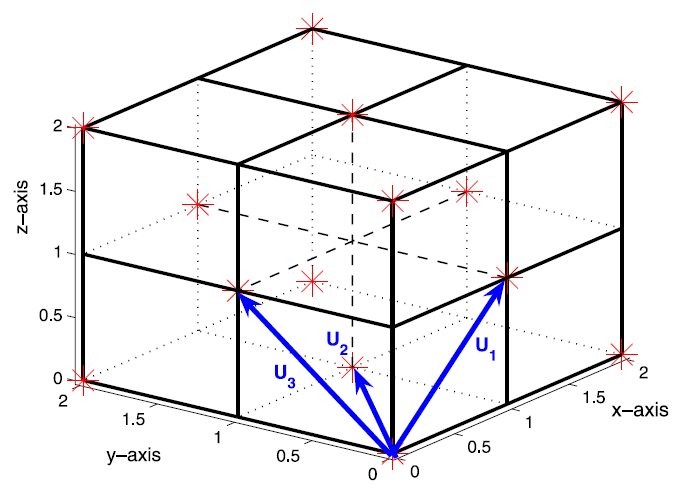
\includegraphics[width=0.4\linewidth]{fcc_basis}
	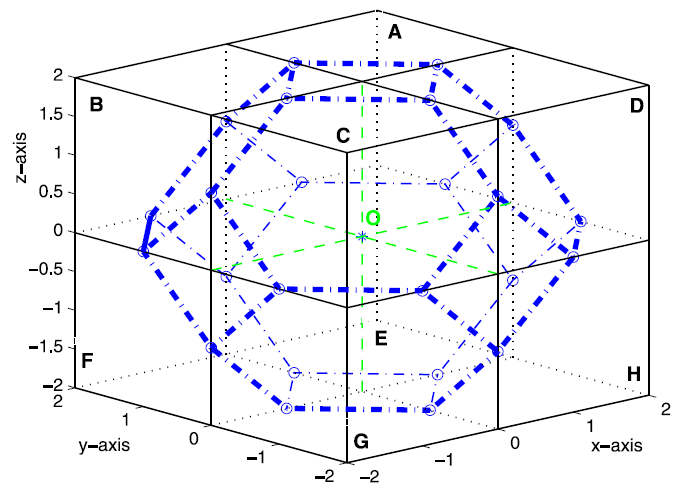
\includegraphics[width=0.4\linewidth]{fcc_voronoi}
	\caption{FCC lattice and its basis vectors and Voronoi cell(truncated octahedron).}
	\label{fig:fcc1}
\end{figure}           
\begin{figure}
	\centering
	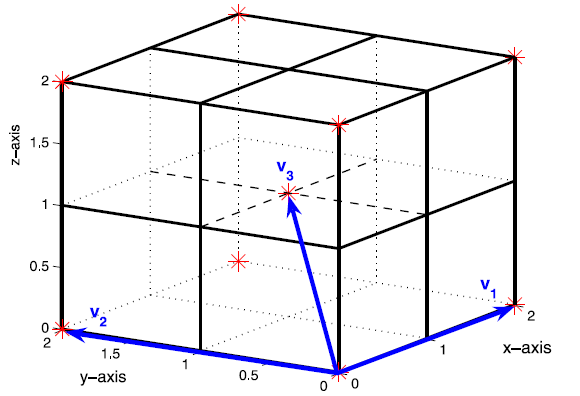
\includegraphics[width=0.4\linewidth]{bcc_basis}
	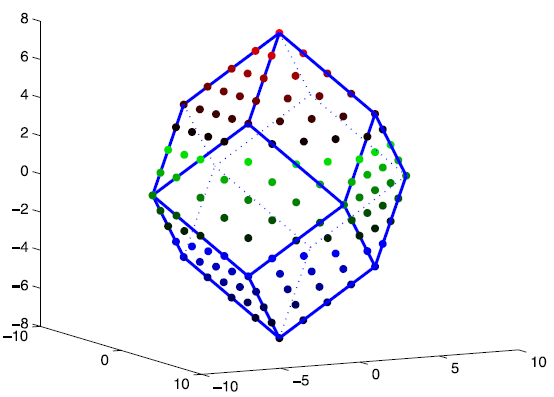
\includegraphics[width=0.4\linewidth]{bcc_voronoi}
	\caption{BCC lattice and its basis vectors and Voronoi cell(rhombic dodecahedron).
	Example corresponds to edge length $4\sqrt{3}a$ ($k=4$).
     }
	\label{fig:bcc1}
\end{figure}
     
   \item ${\bm S}_\Omega$ and ${\bm S}_{\Omega,coef}$:  
     There is no unique choice of coset representatives. 
     One choice is to find non-redundant lattice points (w.r.t. periodicity) 
     in a Voronoi cell centered at the origin.     
     
     Let us denote a set of coset representatives of the quotient group $L/L_0$ as $S_\Omega$.  
     \bea 
     S_\Omega  = \{ {\bm r}| {\bm r}\in L/L_0, {\bm r} \in {\bm \Omega} \}
     \eea 
     In other words, $S_\Omega$ is a set of Cartesian coordinates of lattice points 
     in coset representatives within a Voronoi cell.
     Details on the construction of $S_\Omega$ is explained later.
   
     For each points in $S_\Omega$, there exists a set of corresponding coefficients(lattice coordinates) 
     of basis vectors. The set of coefficients corresponding to $S_\Omega$ are denoted as 
     $S_{\Omega,coef}$,
     \bea 
     S_{\Omega,coef}&=&\{ [{\bm r}] : {\bm U}\cdot[{\bm r}] \in S_\Omega \}.
     \eea   

	\item {\bf Nearest Neighbors}: The number of nearest neighbor points in cubic(FCC,BCC) 
lattice are {\color{red} 6(12,8)} in distance $a(\sqrt{2}a,\sqrt{3}a)$. 
One can find their location from a given lattice point 
by displacements in lattice coordinates $[{\bm r}]$,
\bea 
\Delta \vn_{cubic}&=& (+1,0,0), (-1,0,0), (0,1,0), (0,-1,0),(0,0,1),(0,0,-1),\no  
\Delta \vn_{FCC} &=& (-1,0,0),(-1,0,1),(-1,1,0),(0,-1,0),(0,-1,1),(0,0,-1), \no 
& & (0,0,1),(0,1,-1),(0,1,0),(1,-1,0),(1,0,-1),(1,0,0), \no 
\Delta \vn_{BCC} &=& (-1,0,1),(0,0,1),(0,-1,1),(-1,-1,1),\no 
& & (0,1,-1),(1,1,-1),(1,0,-1),(0,0,-1) . 
\eea 
Next nearest neighbors of cubic(BCC) is 12(6) points.
Next-next nearest neighbors of cubic(BCC) are 8(12) points. 

     
   \item ${\bm S}^A_{\Omega}$ and ${\bm S}^A_{\Omega,coef}$: 
      Frequency set $S^A_{\Omega}$ is a set of coset representatives of 
     $L^*_0/L^*$.(For example, $[N]/N$ in case of 1-D case.)
     \bea 
     S^A_{\Omega}=\{s | s\in  L^*_0/L^* \}.
     \eea 
     
     One can define $S^A_{\Omega,coef}$ such that 
     \bea      
     S^A_{\Omega,coef} &=& \{ [{\bm s}]\in Z^d : (V^T)^{-1}[{\bm s}] \in S^A_\Omega  \}.
     \eea 

  \item  (According to the proposition given in \cite{Zheng}), one can  
       obtain $S^A_{\Omega,coef}$ from $S_{\Omega,coef}$ as
     \bea 
     S^A_{\Omega,coef}&=&\{ A^{-1}c : c\in S_{\Omega,coef} \}.
     \eea         
     According to \cite{Zheng}, unimodular matrix $A$ is defined such that
    \bea 
     & &({\bm V}_{cs}^T)^{-1}=\frac{1}{k}{\bm U}_c\cdot {\bm A}_{cs},\quad 
     ({\bm U}_{c}^T)^{-1}=\frac{1}{k}{\bm V}_{cs}\cdot {\bm A}^T_{cs},\no 
     & & ({\bm V}_{fs}^T)^{-1}=\frac{1}{4k}{\bm U}_f\cdot {\bm A}_{fs},\quad 
     ({\bm U}_{f}^T)^{-1}=\frac{1}{4k}{\bm V}_{fs}\cdot {\bm A}^T_{fs} ,\no 
     & & ({\bm V}_{bs}^T)^{-1}=\frac{1}{4k}{\bm U}_b\cdot {\bm A}_{bs},\quad 
     ({\bm U}_{b}^T)^{-1}=\frac{1}{4k}{\bm V}_{bs}\cdot {\bm A}^T_{bs}.
     \eea  
     Then, 
     \bea 
     {\bm A}_{cs}=\threedmat{1}{0}{0}{0}{1}{0}{0}{0}{1},
     {\bm A}_{fs}=\threedmat{0}{-1}{1}{1}{1}{-1}{-1}{0}{1},
     {\bm A}_{bs}=\threedmat{0}{-1}{1}{-1}{0}{1}{1}{1}{-1},
     \eea                
     It may be defined in a compact way, 
    	\bea 
    	{\bm A}=(|\det{{\bm U}} \det{{\bm V}}|)^{\frac{1}{3}} {\bm U}^{-1}{\bm V}^{-T}, \quad 
    	{\bm V}^{-T}=(|\det{{\bm U}} \det{{\bm V}}|)^{-\frac{1}{3}}{\bm U}{\bm A}
    	\eea 
    {\color{red} However, the proposition about $S^A_{\Omega,coef}$ seems 
    	to be only applicable for above cases.
    (not for other lattice or other periodic boundary condition.)  
    }  
           
   \item {\bf size of $S_\Omega$}: The number of lattice points of $S_\Omega$, $S_{\Omega,coef}$ ,
   $S^A_\Omega$, $S^A_{\Omega,coef}$ for given size parameter $k$ are
   \bea 
   N=\det{\bm D} =\frac{|\det {\bm V}|}{|\det {\bm U}|}\quad\Rightarrow \quad 
   N_{cs}=k^3, \quad N_{fs}=16 k^3,\quad N_{bs}=4 k^3.
   \eea 
   \item ${\bm S}_{\Omega,cartes}$: (this is not in the \cite{Zheng}). 
   we may define a set $S_{\Omega,cartes}$ such that 
   for a ${\bm p}\in S_{\Omega,cartes}$, 
   \bea 
   {\bm p}_i=mod(({\bm E}^{-1}\cdot[\vr])_i,D_{ii} ), \quad [\vr]\in S_{\Omega,coef}
   \eea 
   Now, the ${\bm p}_i$ is in range $[0,D_{ii}-1]$ as like 1-D periodic lattice in i-th direction.
   \footnote{ Be careful that the action of {\bf mod} is different depending on Fortran or MATLAB. 
   	Fortran {\bf modulo} and MATLAB {\bf mod} gives modulo(A,P)$=A-floor(A/P)*P$ which have the same
   	sign of P. 
   	On the other hand Fortran {\bf mod} gives mod(A,P)$=A-int(A/P)*P$ which have the same sign of A. 
   	In both case magnitude are smaller than $|P|$.   
   } 
   Also, in frequency domain, one may define ${\bm w}\in S^A_{\Omega,cartes}$,   
   \bea 
   {\bm w}_i =mod( ({\bm F}^{-T}[{\bm s}] )_i,D_{ii} ), \quad [{\bm s}]\in S^A_{\Omega,coef}.
   \eea 
   
   This is similar to the cubic lattice case. 
   
   Also, because of modular operation, it is easy to find 
   a ${\bm p}\in S_{\Omega,cartes}$ for any lattice point $\vr\notin S_\Omega$. 
   In other words, any two lattice points give the same  ${\bm p}$ are congruent points. 
   
\item {\bf In summary} : For given size parameter $k$ of a lattice and periodicity , 
      $N$ number of lattice points are defined. For $lp-th$ lattice point, 
      there are several representations we can use,
      \bea 
      lp \in [1,N] \quad \leftrightarrow \quad {\bm r} \in S_\Omega 
      \quad \leftrightarrow \quad [{\bm r}] \in S_{\Omega,coef} 
      \quad \leftrightarrow \quad {\bm p} \in S_{\Omega,cartes}
      \eea 
            
\end{itemize}


\section{A Periodic condition in lattice coordinates } 
We may express a lattice points in three coordinates. 
\begin{itemize}
	\item In a Cartesian basis, ${\bm r}=(n_x,n_y,n_z)\in S_{\Omega}$. 
	\item In a Generator basis, ${\bm q}=[{\bm r}]=(q_1,q_2,q_3)\in S_{\Omega,coef}$. 
	\footnote{ ({\color{red} Actually, this should be $q^1,q^2,q^3$ in curvilinear coordinates. 
		But I will ignore the difference from now on.}) }
	\item In a new Cartesian basis, ${\bm p}=(p_1,p_2,p_3)\in S_{\Omega,cartes}$.
\end{itemize}

Any lattice point not in $S_\Omega$ is congruent with a point in $S_\Omega$.
The congruency(periodicity) is easiest to see in ${\bm p}$, we just have 
\bea 
\psi(p_1,p_2,p_3)=\psi(p_1+ D_{11},p_2+ D_{22},p_3+ D_{33})
\eea 
However, the periodicity condition is complicate in other coordinates, 
$f(\vr)=f(\vr')$ for ${\bm r}$ if there exists integers $\vn$ such that 
\bea 
\vr-\vr'={\bm V}{\vn} 
\eea 
or $\phi(\vq)=\phi(\vq')$ for ${\bm q}$ if there exists integers $\vn$ such that
\bea 
\vq-\vq'={\bm U}^{-1}{\bm V}\vn 
\eea 

Thus, probably the easiest way to treat the lattice is to 
always convert between lattice coordinates $\vq$ and $\vp$. 

\subsection{Construction of $S_\Omega$} 
{\color{red} Thus, one way to construct $S_\Omega$ lattice is as follows:}
\begin{itemize}
	\item Construct ${\bm p}=(p_1,p_2,p_3)\in S_{\Omega,cartes}$ with integers 
	     $0\leq p_1\leq D_{11}-1$, $0\leq p_2\leq D_{22}-1$, $0\leq p_3\leq D_{33}-1$.
	\item Convert ${\bm p}$ to $[\vr]$ and ${\vr}$ with appropriate integers 
	      ${\bm n}=(n_1,n_2,n_3)$, 
	     \bea
	     [\vr]&=&{\bm E}\cdot \left({\bm p}-{\bm D}\cdot{\bm n} \right) ,\no 
	     {\bm r}&=& {\bm U}\cdot [\vr]={\bm U}\cdot {\bm E}\cdot \left({\bm p}-{\bm D}\cdot{\bm n} \right). 
	     \eea  
	     However, this conversion is not unique. 
         One way to choose ${\bm n}$ is to minimize the distance $|{\bm r}|$ from the origin. 
         Once ${\bm n}$ is chosen for each ${\bm p}$ points,
         $S_{\Omega}$ and $S_{\Omega,coef}$ can be constructed.
    \item Or, if $S_\Omega$ is easy to construct like cubic lattice. One can obtain $S_{\Omega,coef}$
         and $S_{\Omega,coef}$ by  
         \bea 
           [\vr]&=&{\bm U}^{-1}\cdot \vr , \quad \vr \in S_\Omega,\no 
           {\bm p}_i &=&\mod( ({\bm E}^{-1}[\vr])_i, D_{ii} ) , \quad i=1,2,3.
         \eea 
         
\end{itemize}

\subsection{Distance between two lattice points}
The distance between two points, $\vr_1$ and $\vr_2$, on the lattice have to be 
computed by taking into account periodicity. 
Let us define a function
\bea 
d(\vr,\vn)=\sqrt{(\vr+{\bm V}\cdot\vn)^2}.
\eea 
The distance of two lattice points is the minimum of $d(\vr_1-\vr_2,\vn)$ for given $\vr=\vr_1-\vr_2$ vector.
Question is how to find an integer vector $\vn$ which gives the minimum.  

\subsubsection{Cubic periodic boundary} 
For example, let us consider 1-d periodic lattice of size $N$. 
Let $-\frac{N}{2}\leq x_0< \frac{N}{2}$, $x=x_0+N n$. 
Then for given $x$, we can find $x_0$ and $n$ by 
\bea 
n = \mbox{round}(\frac{x}{N}),\quad x_0=x-Nn.  
\eea 
The same can be applied for cubic periodic boundary condition, where ${\bm V}$ is diagonal,
\bea 
\vn= \mbox{round}({\bm V}^{-1}\vr),\quad \vr_0=\vr-{\bm V}\vn.   
\eea   
where $\mbox{round}$ is implied for each Cartesian component. 
Thus, the distance can be computed simply by $\vr_0^2$.

\subsubsection{BCC/FCC periodic boundary} 
Suppose $\vr\in S_\Omega$ and $\vr'=\vr+{\bm V}\cdot \vn$.
The problem is to find $\vr$ or $\vn$ from given $\vr'$. 
Let us define $\vp'={\bm E}^{-1}{\bm U}^{-1}\vr'$,
\bea 
& &\vr'={\bm U}{\bm E} {\bm p}'= {\bm U}{\bm E} {\bm p}+{\bm V}\cdot\vn ,\no 
&\Rightarrow & {\bm p}' = {\bm p}+{\bm D}\cdot {\bm m},\quad {\bm m}={\bm F}\cdot{\bm n}.  
\eea 
Since ${\bm D}$ is diagonal, we can consider $\vp$ in each component separately. 
However, unlike the cubic lattice, the corresponding range of $\vp$ depends on the 
choice of $S_\Omega$. (In other words, $\vp$ is not necessarily in range $0\leq p_i < D_{ii}$.  )  
For given $\vr'$ or $\vp'$, 
there is a unique $\vp_{0,i}=\mod(\vp'_i,{\bm D}_{ii})$ for  $0\leq p_{0,i} < D_{ii}$
, $\vp_0\in S_{\Omega,cartes}$. 
However, the exact relation between $\vp_0$ and $\vp$ depends on the particular 
choice of $S_\Omega$. Thus, it seems to be difficult to make a simple relation 
like cubic periodic boundary case.  

If we have already tabulated $S_\Omega$, we can make a table of correspondence 
$\vr\leftrightarrow \vp_0$ where $\vr\in S_\Omega$. However, when the lattice size 
parameter is large, this can be slow.

One may shift the $\vr'$ or $\vp'$ by $\vn=\mbox{round}({\bm V}^{-1}\vr')$ or
${\bm m}=\mbox{round}({\bm D}^{-1}\vp') $ first and compare with additional nearby shifts.
This may reduce number of trials. 



\section{Cartesian Periodic boundary condition} 
{\color{red} Sublattice and Periodicity:} One can choose different Sublattice $L_0$
            (this ${\bm V}$ and ${\bm M}$) other than shown in previous section. 
            (This corresponds to divide space into different blocks.
            Previous cubic lattice corresponds to divide space into large periodic cubes.
            On the other hand, previous BCC lattice 
            corresponds to divide space into periodic rhombic dodecahedrons.)   

Imposing Cartesian periodic boundary condition may be easier to use.
Ref. \cite{CD} gives very simple implementation of FFT,which is redundant, 
for cubic periodic boundary condition with BCC/FCC lattice.
Ref. \cite{Zheng} gives non-redundant implementation of FFT for cubic periodic boundary condition
with BCC/FCC lattice. See the appendix for explanation of Ref. \cite{CD}.

Following is the implementation according to Ref. \cite{Zheng}.

\subsection{BCC lattice case}
For  BCC(b) matrix with Cubic(c) sublattice(s) with even integer length $N=2k$, we have
\bea 
{\bm V}_{bcs}:=N \threedmat{1}{0}{0}{0}{1}{0}{0}{0}{1}={\bm U}_b{\bm M}_{bcs},\quad 
{\bm M}_{bcs}:=\frac{N}{2} \threedmat{1}{0}{-1}{0}{1}{-1}{0}{0}{2}.
\eea 
\bea 
{\bm E}_{bcs}=\threedmat{1}{0}{0}{0}{1}{0}{0}{0}{1},\quad 
{\bm D}_{bcs}=k\threedmat{1}{0}{0}{0}{1}{0}{0}{0}{2},\quad 
{\bm F}_{bcs}=\threedmat{1}{0}{-1}{0}{1}{-1}{0}{0}{1}. 
\eea 
One choice of $S_{\Omega}$ is for integers $r,s,t\in Z$,\footnote{
	To make center of Voronoi cell at the origin, for symmetric form, 
    one can use $r,s,t\in [-\frac{N}{4},\frac{N}{4}-1]$ for $S_\Omega$.
} 
\bea 
S_{\Omega}&=&\left\{ \colmthr{2r}{2s}{2t},\colmthr{2r+1}{2s+1}{2t+1} : r,s,t \in [0,\frac{N}{2}-1] \right\},\no 
S_{\Omega,coef}&=&\{ {\bm U}^{-1}{\bm r} : {\bm r}\in S_\Omega\} 
\eea  
For lattice point $\vr={\bm U}[\vr]$, we have\footnote{
 $$ {\bm E}^{-1}_{bcs}= \threedmat{1}{0}{0}{0}{1}{0}{0}{0}{1} \quad 
 {\bm F}^{-T}_{bcs}= \threedmat{1}{0}{0}{0}{1}{0}{1}{1}{1}.$$

}  
\bea 
{\bm E}^{-1}[\vr]=\colmthr{r-t}{s-t}{2t }, \colmthr{r-t}{s-t}{2t+1}.
\eea 
One choice of $S^A_\Omega$ is for integers $u,v,w\in Z$,
\bea 
S^A_\Omega&=& \{ (\frac{u}{N},\frac{v}{N},\frac{w}{N}) :  u,v \in [0,\frac{N}{2}-1], w\in [0,N -1] \}, \no 
S^A_{\Omega,coef}&=& \{ [{\bm s}] : {\bm s}={\bm V}^{-T}[{\bm s}],{\bm s}\in  S^A_\Omega \} 
\eea 
for dual lattice points, ${\bm s}$, $[{\bm s}]$,   
\bea 
{\bm F}^{-T}[{\bm s}]=\colmthr{u}{v}{u+v+w}.
\eea  
By taking modular operation, we have $S_{\Omega,cartes}$ and $S^A_{\Omega,cartes}$ and these
can be used for DFT. 

{\bf Note:} Construction of $S_{\Omega}$ which is symmetric w.r.t. the origin is easy.
However, it is not trivial for me to construct $S^A_\Omega$ if one wants to make it symmetric to the origin
such that  $-\frac{N}{2}\leq u,v,w< \frac{N}{2}-1 $ and close to the $(0,0,0)$. 
We may follow following algorithm to construct $S^A_\Omega$ which is symmetric to the origin.
\begin{itemize}
	\item (1) Any combination of $(u,v,w)$, $u,v \in [0,\frac{N}{2}-1], w\in [0,N -1]$ is unique. 
	
	\item (2) test following cases for a $(u,v,w)$,
	\bea 
	& &(u,v,w-N),(u,v-N,w),(u-N,v,w),(u,v-N,w-N),(u-N,v,w-N) \no 
	& & (u-\frac{N}{2},v-\frac{N}{2},w),
	    (u-\frac{N}{2},v,w-\frac{N}{2}),(u,v-\frac{N}{2},w-\frac{N}{2}), \no 
	& & (u-\frac{N}{2},v-\frac{N}{2},w-N)
	\eea     
	\item (3) Choose one of them which is closest to the origin. 
\end{itemize}


\subsection{FCC lattice case}
For  FCC(f) matrix with Cubic(c) sublattice(s) with even integer length $N=2k$, we have
\bea 
{\bm V}_{fcs}:=N\threedmat{1}{0}{0}{0}{1}{0}{0}{0}{1}={\bm U}_b{\bm M}_{fcs},\quad 
{\bm M}_{fcs}:=\frac{N}{2} \threedmat{1}{-1}{1}{1}{1}{-1}{-1}{1}{1}.
\eea 
\bea 
{\bm E}_{fcs}=\threedmat{1}{0}{0}{1}{1}{-1}{-1}{0}{1},\quad 
{\bm D}_{fcs}=k\threedmat{1}{0}{0}{0}{2}{0}{0}{0}{2},\quad 
{\bm F}_{fcs}=\threedmat{1}{-1}{1}{0}{1}{0}{0}{0}{1}. 
\eea 
One choice of $S_{\Omega}$ is for integers $r,s,t\in Z$,
\bea 
S_{\Omega}&=&\left\{ {\bm r} : {\bm r}=
\colmthr{2r}{2s}{2t},\colmthr{2r}{2s+1}{2t+1}, \colmthr{2r+1}{2s}{2t+1},\colmthr{2r+1}{2s+1}{2t} 
   ,\quad  r,s,t \in [0,\frac{N}{2}-1]\right\},\no 
S_{\Omega,coef}&=&\{ {\bm U}^{-1}{\bm r} : {\bm r}\in S_\Omega\} 
\eea  
For a lattice point ${\bm U}[\vr]$, we have\footnote{
$${\bm E}^{-1}_{fcs}= \threedmat{1}{0}{0}{0}{1}{1}{1}{0}{1},\quad 
  {\bm F}^{-T}_{fcs}= \threedmat{1}{0}{0}{1}{1}{0}{-1}{0}{1}.
$$.
}  
\bea 
{\bm E}^{-1}[\vr]=\colmthr{r-s+t}{2s}{2t},\colmthr{r-s+t}{2s+1}{2t+1},
                                        \colmthr{r-s+t+1}{2s}{2t+1},\colmthr{r-s+t}{2s+1}{2t}.
\eea 
One choice of $S^A_\Omega$ is for integers $u,v,w\in Z$,
\bea 
S^A_\Omega&=& \{ (\frac{u}{N},\frac{v}{N},\frac{w}{N}) :  u \in [0,\frac{N}{2}-1], v,w\in [0,N-1] \}, \no 
S^A_{\Omega,coef}&=& \{ [{\bm s}] : {\bm s}={\bm V}^{-T}[{\bm s}],{\bm s}\in  S^A_\Omega \} 
\eea 
\bea 
{\bm F}^{-T}[{\bm s}]=\colmthr{u}{v+u}{w-u}.
\eea  

Note that above relations will be satisfied for any other choice of $S_\Omega$ or $S^A_\Omega$
as long as they are coset representatives of $P$ and $\hat{P}$. 
Note that \cite{Zheng} have errors/typo in the algorithm.  

{\bf Note:} Construction of $S_{\Omega}$ which is symmetric w.r.t. the origin is easy.
However, it is not trivial to construct $S^A_\Omega$ if one wants to make it symmetric to the origin
such that  $-\frac{N}{2}\leq u,v,w< \frac{N}{2}-1 $ and close to the $(0,0,0)$. 
We may follow following algorithm.

(1) Any combination of $(u,v,w)$, $u\in [0,\frac{N}{2}-1], v, w\in [0,N -1]$ is unique. 

(2) Test following cases for given $(u,v,w)$.
\bea 
& &(u-N,v,w), (u,v-N,w),(u,v,w-N),\no 
& &(u-\frac{N}{2},v-\frac{N}{2},w-\frac{N}{2})
\eea 

(3) Choose one of them which is closest to the origin. 
 
\chapter{BCC lattice} 

\section{BCC lattice} 
BCC(Body-centered-cubic) lattice 
can be generated from the three column vectors of ${\bm U}_b$, 
and size of Voronoi cell is determined by $k$ in
FCC sublattice generators ${\bm V}_{bs}$.
\bea       
{\bm U}_b=\threedmat{2}{0}{1}{0}{2}{1}{0}{0}{1},\quad {\bm V}_{bs}=k\threedmat{2}{0}{2}{0}{2}{2}{2}{2}{0}
\eea 
This implies that two points 
$\vr$ and $\vr'$ are congruent, 
if there exits some integers ${\bm n}$ such that
\bea 
\vr'=\vr+{\bm V}_{bs}\cdot {\bm n}
\eea 
This is equivalent to the existence of integers $(n_x,n_y,n_z)$ or  $(n_1,n_2,n_3)$ such that 
\bea 
\colmthr{x'}{y'}{z'}-\colmthr{x}{y}{z}= 2k \colmthr{n_x+n_z}{n_y+n_z}{n_y+n_x}=
2k \colmthr{n_1}{n_2}{n_1+n_2-2 n_3}
\eea 
In other words, two points are congruent if,
\bea 
\mbox{mod}(x',2k)=\mbox{mod}(x,2k),\quad 
\mbox{mod}(y',2k)=\mbox{mod}(y,2k),\quad 
\mbox{mod}(x'+y'+z',4k)=\mbox{mod}(x+y+z,4k).\nonumber  
\eea 

Any BCC lattice coordinate $[\vr]$ in non-orthogonal basis
can be converted into Cartesian coordinates 
\bea 
\colmthr{x}{y}{z}={\bm U}_b\cdot[\vr]=\colmthr{2[\vr]^1+[\vr]^3}{2[\vr]^2+[\vr]^3}{[\vr]^3}
\eea 

Thus, two BCC lattice coordinates $c$ and $c'$ are 
	congruent if there exists integers which satisfies
	$U_b{\bm c}'=U_b{\bm c}+V_{bs}\cdot {\bm n}$
	\bea 
	\colmthr{c^1}{c^2}{c^3}'-\colmthr{c^1}{c^2}{c^3} &=& k \colmthr{-n_2+n_3 }{-n_1+n_3 }{2n_1+2n_2 }
	=k \colmthr{-n'_1}{-n'_2}{4n'_3+2n'_1+2n'_2}
	\eea 
	In other words, the congruency test in BCC coordinate is\footnote{ 
		For a comparison, the congruency test in FCC coordinate is
		\bea 
		\mbox{mod}(c^{'1},k)=\mbox{mod}(c^{'2},k),\
		\mbox{mod}(c^{'2}-c^{'1},4k)=\mbox{mod}(c^{2}-c^{1},4k),\
		\mbox{mod}(c^{'3}-c^{'2},4k)=\mbox{mod}(c^{3}-c^{2},4k).
		\eea 
	} 
	\bea 
	\mbox{mod}(c^{'1},k)=\mbox{mod}(c^1,k),\ 
	\mbox{mod}(c^{'2},k)=\mbox{mod}(c^2,k),\quad 
	\mbox{mod}(2c^{'1}+2c^{'2}+c^{'3},4k)=\mbox{mod}(2c^1+2c^2+c^3,4k) \nonumber 
	\eea  

\subsection{metric tensor} 
covariant basis vectors are, 
\bea 
{\bm u}_1=2\hat{e}_x \quad 
{\bm u}_2=2\hat{e}_y ,\quad
{\bm u}_3= \hat{e}_x+\hat{e}_y+\hat{e}_z.
\eea 
And contravariant basis vectors
\bea 
{\bm u}^1=\frac{1}{2}\hat{e}_x-\frac{1}{2}\hat{e}_z,\quad 
{\bm u}^2=\frac{1}{2}\hat{e}_y-\frac{1}{2}\hat{e}_z,\quad 
{\bm u}^3=\hat{e}_z.
\eea 
Also we get metrics,\footnote{$\det(g)=16$}
\bea 
g_{ij}=\threedmat{4}{0}{2}{0}{4}{2}{2}{2}{3},\quad 
g^{ij}=\threedmat{\frac{1}{2}}{\frac{1}{4}}{-\frac{1}{2}}
{\frac{1}{4}}{\frac{1}{2}}{-\frac{1}{2}}
{-\frac{1}{2}}{-\frac{1}{2}}{1}
\eea

\subsection{Laplacian and others} 
A Laplacian in BCC lattice coordinate is
\bea 
\nabla^2 \psi&=& g^{ki}\frac{\del^2\psi}{\del q^k \del q^i} \no 
             &=&\left[ \frac{1}{2}(\frac{\del}{\del q^1})^2+\frac{1}{2}(\frac{\del}{\del q^2})^2
+ \frac{1}{2}(\frac{\del^2}{\del q^1 \del q^2})
+(\frac{\del}{\del q^3})^2-\frac{\del^2}{\del q^1 \del q^3}  
-\frac{\del^2}{\del q^2 \del q^3}
\right]\psi                             
\eea 

Jacobian is ${\color{red} J=4}$, thus
\bea 
d^3 x = 4 d q^1 d q^2 d q^3
\eea 
gradient (We may use Cartesian basis for spin and iso-spin)
\bea 
{\bm \sigma}\cdot\nabla \pi = \sigma^i \frac{\del \pi}{\del q^i}
\eea 
where 
\bea 
\colmthr{\sigma^1}{\sigma^2}{\sigma^3}={\bm U}_{b}^{-1}\colmthr{\sigma^x}{\sigma^y}{\sigma^z}
= \threedmat{\frac{1}{2}}{0}{-\frac{1}{2}}{0}{\frac{1}{2}}{-\frac{1}{2}}{0}{0}{1}
\colmthr{\sigma^x}{\sigma^y}{\sigma^z}
\eea 

\section{Discrete Fourier Transform on a BCC lattice}

\subsection{Construction $S_{\Omega,coef}$}
A Voronoi cell  $\Omega$ centered at ${\bm 0}$ is  
\bea 
\Omega:=\left\{\colmthr{x}{y}{z}: |x|+|y|< 2k,\ |x|+|z|< 2k,\ |y|+|z|< 2k \right\}
\eea 
The condition for BCC lattice points $\Xi=\Omega\cap L_b$ are, in terms of lattice coordinates,
${\bm c}\in S_{\Omega,coef}$, 
\bea 
& & -k\leq c_1 \leq k,\no 
& &\max\{-k,c_1-k\}\leq c_2 \leq \min\{k,c_1+k\},\no 
& &\max\{-k-c_1-c_2,-k-c_1,-k-c_2\}\leq c_3 \leq \min\{k-c_1-c_2,k-c_1,k-c_2\}.
\eea 

(In fact, as long as $S$ becomes a coset representative of $L/L_0$, 
the choice of $S$ or $S_{coef}$ is arbitrary. 
One of the simplest way to construct $S_{\Omega,coef}$
is to choose $0\leq c_1\leq k-1$, $0\leq c_2\leq k-1$, $0\leq c_3\leq 4k-1$.
However, the shape of $S$ will not be centered on the origin
and the shape becomes a skewed cubic.)

If we denote $\vp={\bm E}^{-1}\cdot c$, we have 
\bea 
& & p_1=-c_2,\quad p_2=-c_1,\quad p_3=2c_1+2c_2+c_3,\no 
&\Rightarrow &-k\leq p_2\leq k,\no 
& & -\min\{k,-p_2+k\}\leq p_1 \leq -\max\{-k,-p_2-k\},\no 
& & \max\{-k+p_1+p_2,-k+p_2,-k+p_1\}-2p_2-2p_1 \no 
& &\quad \leq p_3 \leq \min\{k+p_1+p_2,k+p_2,k+p_1\}-2p_2-2p_1.
\eea 
{\bf Note:} Though the range of $p_i$ are given. 
not all values of $p_i$ are independent.( $p_i$ and $p'_i$ is equivalent if 
$p'_i=p_i+D_{ii}n$. )


The lattice points with Voronoi cell, $\Xi$
can be constructed with the algorithm given in 
Zheng's paper\cite{Zheng} which is searching BCC lattice points within $\Omega$.
The algorithm generates $\Xi$ which have 
$(4k^3+6k^2+4k+1)$ number of lattice points. 
However, one have to remove redundant points to obtain coset representative $S_{\Omega}$ 
of the quotient group and the explicit algorithm for  $S_{\Omega,coef}$ is not given in \cite{Zheng}. (One choice of  $S_{\Omega,coef}$ is given in the Appendix. )

After removing redundant congruent points on the surface or edge
 , one gets $4k^3$ number of lattice points, $S_{\Omega,coef}$,
\bea 
S_{\Omega,coef}:=\{ {\bm c}: {\bm U}_b\cdot{\bm c}\in S_\Omega \}.
\eea  
Corresponding frequency domain can be obtained by 
\bea 
S^A_{\Omega,coef}=\{A^{-1}{\bm c}:{\bm c}\in S_{\Omega,coef} \},\quad 
{\bm A}=\threedmat{0}{-1}{1}{-1}{0}{1}{1}{1}{-1}
\eea 

{\bf FCC lattice case:} Similar $S_{\Omega,coef}$ condition for FCC lattice is 
\bea 
& & -\frac{3}{2}k\leq c_1\leq \frac{3}{2}k, \no 
& & \max\{-\frac{3}{2}k,-2k-c_1\}\leq c_2 \leq \min\{\frac{3}{2}k,2k-c_1\},\no 
& & \max\{-\frac{3}{2}k-c_1-c_2,-\frac{3}{2}k,-2k-c_1,-2k-c_2\}\leq c_3
    \leq \min\{\frac{3}{2}k-c_1-c_2,\frac{3}{2}k,2k-c_1,2k-c_2\}.  \nonumber 
\eea 
Also, for $\vp={\bm E}^{-1}\cdot c$,
\bea 
& &p_1=c_1,\quad p_2=-c_1+c_2,\quad p_3=-c_2+c_3,\no 
&\Rightarrow & -\frac{3}{2}k\leq p_1\leq \frac{3}{2}k, \no 
& & \max\{-\frac{3}{2}k,-2k-p_1\}-p_1\leq p_2 \leq \min\{\frac{3}{2}k,2k-p_1\}-p_1,\no 
& & \max\{-\frac{3}{2}k-2p_1-p_2,-\frac{3}{2}k,-2k-p_1,-2k-p_1-p_2\}-p_1-p_2 \no
 & &\quad \leq p_3 \leq \min\{\frac{3}{2}k-2p_1-2_2,\frac{3}{2}k,2k-p_1,2k-p_1-p_2\}-p_1-p_2. 
\eea 

\subsection{algorithm of FFT on lattice}
Let us suppose the indexing for position space and frequency domain is done as follows.
\bea 
S_{\Omega} &:=&\{{\bm r}: \mbox{A coset representative of quotient group } L/L_0 \},\no 
S_{\Omega,coef}&:=&\{ [{\bm r}] : {\bm U}\cdot[{\bm r}] \in S_{\Omega} \},\no 
S^A_{\Omega,coef}&:=&\{{\bm A}^{-1}{\bm c}: {\bm c}\in S_{\Omega,coef}\},\no 
S^A_{\Omega}&:=&\{{\bm s}: \mbox{A coset representative of quotient group } L_0^*/L^*  \},\no
&=&\{({\bm V}^T)^{-1}{\bm c} :{\bm c}\in  S^A_{\Omega,coef}    \}
\eea 
we can express these as $3\times 4k^3$ matrix (like $S_{\Omega,coef}(1:3,1:4k^3)$)
such that each column vector corresponds to one point. 

Suppose $f_{in}(l)$ is defined on $1\leq l\leq 4k^3$
such that $f_{in}(l)$ is evaluated at l-th column vector of  $S_{\Omega,coef}$.
We can obtain corresponding DFT on BCC lattice, $f_{in}\to \hat{f}$, 
where $\hat{f}(l)$ is defined on l-th column vector of $S^A_{\Omega,coef}$,
by using usual DFT from the fact,  
\bea 
\la {\bm r},{\bm s}\ra ={\bm r}^T\cdot{\bm s}
&=&[{\bm r}]^T\cdot({\bm M}^{-1})^T\cdot[{\bm s}]_{\tilde V} \no 
&=& \left( {\color{red}E^{-1}}[{\bm r}]\right)^T  D^{-1} \left( (F^{-1})^T[{\bm s}]_{\tilde V} \right). 
\eea 

For each $1\leq l\leq 4k^3$, we can associate $(p,q,r)={\color{red}E^{-1}}[{\bm r}]_l$ with modular $(k,k,4k)$
and define $f(p,q,r)=f_{in}(l)$. 
(then p and q in range $(0,k-1)$ and r in range $(0,4k-1)$).
Let us denote such points as $S_{\Omega,cartes}$ and 
also $S^A_{\Omega,cartes}$ in frequency similarly.
\bea 
S_{\Omega,cartes}&:=&\{{\color{red}E^{-1}}[{\bm r}] : [r]\in S_{\Omega,coef}  \},\no 
S^A_{\Omega,cartes}&:=&\{(F^{-1})^T[{\bm s}]_{\tilde V} : [s]_{\tilde V}\in S^A_{\Omega,coef} \}
\eea 

The FFT of $f_{in}$ can be done with the algorithm given in \cite{Zheng}: 
\begin{itemize}
	\item[(1)] For each $l$, find $(p,q,r)\in S_{\Omega,cartes}$ corresponding to $[{\bm r}]_l\in S_{\Omega,coef}$ 
	and put $f_{cartes}(p,q,r)=f_{in}(l)$
	\item[(2)] Do DFT as usual with $f_{cartes}\to \hat{f}_{cartes}$.
	\item[(3)] For each $l$, find $(p,q,r)\in S^A_{\Omega,cartes}$ corresponding to $[{\bm s}]_l\in S^A_{\Omega,coef}$
	and put $\hat{f}(l)=\hat{f}_{cartes}(p,q,r)$.
\end{itemize}

Some comments: 
\begin{itemize} 
	\item size of lattice is determined by integer $k$ such that number of lattice points
	$L=4k^3$.
	\item $BCCfftBCCout(S_{\Omega,coef},f_{in})$ 
	returns $\hat{f}_{out}$ which is FFT components. 
	It is equivalent to
	\bea 
	\hat{f}_{out}(n)=\sum_{m=1}^{L} f_{in}(m) e^{-2\pi i {\bm [c]}^T_{m}\cdot(M^{-1})^T\cdot {\bm [s]}_{n}}
	\eea   
	where ${\bm [c]}_m$ is a point in $S_{\Omega,coef}$
	and ${\bm [s]}_n$ is a point in $S^A_{\Omega,coef}$
	
	\item $iBCCfftBCCout(S_{\Omega,coef},\hat{f}_{in})$ 
	returns $f_{re}$ from
	\bea 
	f_{re}(n)=\frac{1}{L}\sum_{m=1}^{4k^3} \hat{f}_{in}(m) e^{2\pi i {\bm [c]}^T_{n}\cdot(M^{-1})^T\cdot {\bm [s]}_{m}}
	\eea 
	\item 
	Note that for using FFTW algorithm, one have to divide the output with $L=4k^3$. 	
	\item Note that the corresponding momentum $p_i=-i\nabla_{q_i}$ is from  
	\bea 
	\la {\bm r}_m,{\bm s}_n\ra={[\bm r]}_m^T\cdot (M^{-1})^T\cdot {\bm [s]}_{n}
	\eea 
	where $[\bm r]\in S_{\Omega,coef}$ and ${\bm [s]}\in S_{\Omega,coeff}^A$.
	\footnote{ 
	In curvilinear coordinate convention,
	\bea 
	   (q^1,q^2,q^3)\leftrightarrow [\vr], \quad 
	   (p_1,p_2,p_3)=-i (\frac{\del}{\del q^1},\frac{\del}{\del q^2},\frac{\del}{\del q^3})
	   \leftrightarrow 2\pi (M^{-1})^T\cdot {\bm [s]}
	\eea 
    }
	In other words, $2\pi (M^{-1})^T\cdot {\bm [s]}_{n}$ corresponds to derivative
	(or momentum) ${\bm p}=-i\nabla_{q}$.	
\end{itemize} 






\section{Numerical Derivatice in BCC lattice}
For the derivative, we may use simple approximation 
\bea 
\frac{\del \psi({\bm q})}{\del q^i}\simeq \frac{\psi(q^i+\Delta)-\psi(q^i-\Delta)}{2\Delta}
\eea 
For in ${\bm u}_3$ direction, this derivative use nearest neighbor points, $\Delta={\color{red}\sqrt{3}}a$.
However, in ${\bm u}_{1,2}$ direction, they are not using nearest neighbor points.
Thus, it may be better to use those nearest neighbor points for derivative approximation.
 
Let us use lattice points index $n_i$ such as
$q^{1,2}=2a n_{1,2}$ and $q^3={\color{red}\sqrt{3}}a n_3$,
from the displacement for 8 nearest neighbors are
\bea 
\Delta \vn= (0,0,1),(0,-1,1),(1,0,-1),(1,1,-1),(-1,0,1),(0,1,-1),(0,0,-1),(-1,-1,1)
\eea, 
One possible form is
\bea 
\frac{\del \psi_{n_1,n_2,n_3} }{\del q^1}&\simeq &
   \frac{1}{{\color{red} 2} a}\Big[ \frac{1}{4}
               (\psi_{n_1, n_2,n_3+1} +\psi_{n_1,n_2-1,n_3+1}
         +\psi_{n_1+1,n_2,n_3-1}+\psi_{n_1+1,n_2+1,n_3-1})
   \no & &
  -\frac{1}{4}(\psi_{n_1-1,n_2,n_3+1}+\psi_{n_1,n_2+1,n_3-1}
    +\psi_{n_1,n_2,n_3-1}+\psi_{n_1-1,n_2-1,n_3+1}) \Big] 
\eea 
while 
\bea 
\frac{\del \psi_{n_1,n_2,n_3} }{\del q^3}&\simeq &
  \frac{1}{{\color{red} 2\sqrt{3}} a}\left[\psi_{n1,n2,n3+1}-\psi_{n1,n2,n3-1} \right]  
\eea 

It may be more easier to use DFT to compute derivatives.
(Obtain $\hat{f}_k$ from DFT of $f(n)$. Multiply momentum factors 
to $\hat{f}_k$. Then inverse DFT to get $\nabla f(n)$.)
However, it should be noted that computing derivative using DFT
only works for periodic functions. If the function does not satisfy the 
periodic condition, the results would have errors. 

\section{Free Hamiltonian in BCC lattice}

The free action becomes
\bea 
& &\int dt \int_V d^3 x \frac{-1}{2m}\psi^\dagger(x)\nabla^2\psi(x) \no 
&=&\int dt \int_{S_{\Omega,coeff}} {\color{red}4} d^3 q \frac{-1}{2m} \psi^\dagger({\bm q})\left[ \frac{1}{2}(\frac{\del}{\del q^1})^2+\frac{1}{2}(\frac{\del}{\del q^2})^2
+ \frac{1}{2}(\frac{\del^2}{\del q^1 \del q^2})
+(\frac{\del}{\del q^3})^2-\frac{\del^2}{\del q^1 \del q^3}  
-\frac{\del^2}{\del q^2 \del q^3}
\right]\psi({\bm q}) \no 
&\to& a_t \sum_{n_t} (4a^3) \sum_{{\bm q}_n} 
    \frac{-1}{2m} \psi^\dagger({\bm q}_n)\left[ \frac{1}{2}(\frac{\del}{\del q^1})^2+\frac{1}{2}(\frac{\del}{\del q^2})^2
    + \frac{1}{2}(\frac{\del^2}{\del q^1 \del q^2})
    +(\frac{\del}{\del q^3})^2-\frac{\del^2}{\del q^1 \del q^3}  
    -\frac{\del^2}{\del q^2 \del q^3}
    \right]\psi({\bm q}_n) \nonumber 
\eea 

After Fourier transformation, this becomes
\bea 
&\to& a_t \sum_{n_t} (4a^3) (L)\sum_{{\bm p}_n} 
\frac{1}{2m} \hat{\psi}^\dagger({\bm p}_n)(\frac{1}{2} p_{n,1}^2+\frac{1}{2}p_{n,2}^2+\frac{1}{2}p_{n,1} p_{n,2}
+p_{n,3}^2-p_{n,1} p_{n,3}-p_{n,2} p_{n,3}) \hat{\psi}({\bm p}_n) \nonumber 
\eea 
where $(L=4k^3)$ factor can be absorbed into $\hat{\psi}^\dagger(p)$ and $\hat{\psi}(p)$
depending on the convention of DFT. 

We may compute free action by using DFT,(instead of approximate numerical derivative), as follows
\begin{itemize}
	\item Define 
	\bea 
	\Phi({\bm q}_n)\equiv -\left[ \frac{1}{2}(\frac{\del}{\del q^1})^2+\frac{1}{2}(\frac{\del}{\del q^2})^2
	+ \frac{1}{2}(\frac{\del^2}{\del q^1 \del q^2})
	+(\frac{\del}{\del q^3})^2-\frac{\del^2}{\del q^1 \del q^3}  
	-\frac{\del^2}{\del q^2 \del q^3}
	\right]\psi({\bm q}_n)
	\eea 
	\item First do FFT of $\psi({\bm q}_n)$, to get $\hat{\psi}({\bm p_m})$
	\bea 
	   \hat{\psi}({\bm p_n})= \sum_{{\bm q}_n} {\psi}({\bm q_n}) e^{-i {\bm q}_n\cdot {\bm p}_n },\quad 
	   \psi({\bm q}_n)=\frac{1}{L}\sum_{{\bm p}_n} \hat{\psi}({\bm p_n}) e^{i {\bm q}_n\cdot {\bm p}_n }
	\eea 
	\item compute 
	\bea 
	 \hat{\Phi}({\bm p}_n) &=& p_i g^{ij} p_j \hat{\psi}({\bm p}_n) \no 
	   &=&\left( (\frac{p_1}{2})^2+(\frac{p_2}{2})^2+(-\frac{p_1}{2}-\frac{p_2}{2}+p_3)^2 \right)\hat{\psi}({\bm p}_n) 
	\eea 
	\item inverse transform $\hat{\Phi}({\bm p}_n)$, to get $\Phi({\bm q}_n)$
	\bea 
	 \Phi({\bm q}_n)=\frac{1}{L}\sum_{{\bm p}_n} \hat{\Phi}({\bm p_n}) e^{i {\bm q}_n\cdot {\bm p}_n }
	\eea
	\item Then free particle action becomes
	\bea 
    \int dt \int_V d^3 x \frac{-1}{2m}\psi^\dagger(x)\nabla^2\psi(x)  
	&\to& a_t \sum_{n_t} (4a^3) \sum_{{\bm q}_n} 
	\frac{1}{2m} \psi^\dagger({\bm q}_n)\Phi({\bm q}_n)
	\eea  
	\item Note the factor $4a^3$ in the action. This implies that when we compute the action we have to multiply $4a^3$ for the $H_{free}$ term. This factor will appear in every part of the action. But it is possible to absorb this factor in the normalization
	of fields $\sqrt{4a^3}\psi(x)\to \psi(x)$ which only change overall normalization in path integral $\int{\cal D}\psi$. Thus, it does not affect the lattice calculation.  
\end{itemize}	

\subsection{Dispersion relation of a free particle on lattice}\label{sec:dispersion} 
Let us consider a spectrum of free particle in a periodic BCC lattice.

Obviously, the lowest energy free particle state is  ${\bm p}={\bm 0}$ with $p^2=0$.

From the periodicity condition, possible values of
${\bm p}=(p_x,p_y,p_z)$ must satisfy for any integers ${\bm n}=(n_1,n_2,n_3)$,
\bea 
{\bm p}^T \cdot {\bm V}{\bm n}=2\pi(\mbox{integer}).
\eea 
This condition can be satisfied for BCC lattice if 
\bea 
p_x+p_z=\frac{2\pi}{2k}(\mbox{integer}),\quad 
p_y+p_z=\frac{2\pi}{2k}(\mbox{integer}),\quad 2 p_z=\frac{2\pi}{2k}(\mbox{integer}).
\eea 
In other words, momentums in BCC lattice are 
\bea 
{\bm p}&=&\frac{2\pi}{4k}(m_x,m_y,m_z), \quad 
p^2=(\frac{2\pi}{4k})^2(m_x^2+m_y^2+m_z^2)
\eea 
where integers $m_{x,y,z}$ have the same parity(all even or all odd). 

Similary, for FCC lattice, the condition can be satisfied if
\bea 
2p_x=\frac{2\pi}{2k}(\mbox{integer}),\quad 
2p_y=\frac{2\pi}{2k}(\mbox{integer}),\quad 
p_x+p_y+p_z=\frac{2\pi}{2k}(\mbox{integer}).
\eea 
In other words, momentums in FCC lattice are 
\bea 
{\bm p}=\frac{2\pi}{4k}(m_x,m_y,m_z)
\eea 
where $m_x+m_y+m_z$ is an even number. 

Thus, first excited state of free particle in BCC have  
$p^2=3(\frac{2\pi}{4k})^2$ while 
$p^2=2(\frac{2\pi}{4k})^2$  for FCC, $p^2=(\frac{2\pi}{k})^2$ for cubic. 
(In the code, one can find all possible momentum values $(p_1,p_2,p_3)$
from $S_{freq,coef}$.)

By using this fact, one can construct 
a periodic initial wave function in BCC(FCC) lattice
coordinates , with momentum 
${\bm p}=(p_x,p_y,p_z)$ satisfying above conditions,
\bea 
e^{i{\bm r}^T \cdot {\bm p} }=e^{i [{\bm q}]^T \cdot{\bm U}^T{\bm p} }
\eea 
 
Or, more simply, one can use a symmetric function $f(\vr)$ centered at the origin
with vanishing tail for an initial wave with zero momentum .

\chapter{Numerical realization in nuclear lattice code} 
Unlike the simple Cartesian lattice, in which $S_\Omega=S_{\Omega,coef}$,
for BCC or FCC, one have to choose how the single particle wave function of nucleon or 
auxiliary particle(and pion) configuration should be represented 
in the code. There may be three possible choices(Also for frequency domain).
\begin{itemize}
	\item ${\bm r}\in S_{\Omega}$: This is the same as the Cartesian lattice, 
	                               but all functions $f({\bm r})$
	                               have to be evaluated only on $S_{\Omega}$. 	                               
	      {\bf Note:} To work with DFT on lattice, the function should satisfy the periodicity.
	                  Thus, one have to be careful to define initial waves on lattice.    	                               
	\item $[{\bm r}]\in S_{\Omega,coef}$ : One construct a index matrix $3\times$({lattice size}), 
	       ${\bm S}_{\Omega,coef}$, and evaluate functions $g([{\bm r}]_l)$
	       at l-th column vectors of index matrix. (Or in Cartesian coordinates, $g([{\bm r}]_l)=f(\vr_l)$ 
	       This would be a natural choice of BCC lattice formulation.
\end{itemize}
  
  I will use the $[{\bm r}]\in S_{\Omega,coef}$ for coordinates in the lattice code.
As a test case, let us modify the {\bf nuclei} code to use {\bf lattice\_fft} codes
for a cubic lattice.
The key subroutine of {\bf nuclei} for transfer matrix calculation 
is {\bf getzvecs} and {\bf getzdualvecs}. 
For cubic lattice, by adding a layer of conversion in front and end of using 
{\bf lattice\_fft} code, I can replace these subroutines into a  {\bf lattice\_fft} subroutines. 

Though {\bf nuclei} and {\bf lattice\_fft} use both the cubic lattice , 
because they use different range of index,
one needs conversion. 
\bea 
& &\mbox{zvecs}(n_x,n_y,n_z)\leftrightarrow \mbox{zvecs}(l),\no 
& & n_{x,y,z}\to  q_{1,2,3}=n_{x,y,z}-L*\mbox{int}(2*n_{x,y,z}/L) , \no 
& & q_{1,2,3} \to n_{x,y,z}=\mbox{mod}(q_{1,2,3}+L,L). 
\eea 

\section{init\_lattice} 
The {\bf init\_lattice} initialize the lattice.
\begin{itemize}
	\item lattice\_type and lsize\_k gives lattice\_size
	
	\begin{tabular}{c c c c c}
		type & description               & lattice\_size  & 1d-period & Voronoi cell\\
		\hline
		1    & cubic with cubic boundary &  $k^3$     &    $k$  & cube  \\
		2    & BCC with FCC boundary     &  $4k^3$    &         & rhombic dodecahedron  \\
		3    & FCC with BCC boundary     &  $16k^3$   &         & truncated octahedron  \\
		4    & BCC with cubic boundary   &  $2k^3$    &   $2k$  & cube   \\
		5    & FCC with cubic boundary   &  $4k^3$    &   $2k$  & cube  \\ 
	\end{tabular}

    \item nSomega : list of Cartesian coordinates of non-redundant lattice points. The origin is at the center. 
    \item nSomega\_coef : list of coordinates in lattice generating vector basis of lattice points.  
    \item get\_congruent : return lattice index which is equivalent to the input lattice point. 
    \item \dots 
	
\end{itemize}


\section{getzvecs }  
\begin{itemize}
	\item The free action in {\bf nuclei} code used "improved action" 
	while  it is better to use FFT in {\bf lattice\_fft} code. Thus the exact numerical
	comparison requires additional consideration of dispersion relation. 
	\item {\color{red} Discussion on center of mass coordinate on lattice is necessary. } 
                          
    \item For the free action part, it is calculated in following way.
        Assume a s.p. state $|\vn\ra$, $|f\ra$, s.p. wave functions $f(\vn)$
     such that  
      \bea 
         |\vn\ra= a^\dagger(\vn)|0\ra,\quad \la \vn|f\ra=  \la 0| a(\vn)|f\ra= f(\vn).
      \eea 
      Then, the transfer matrix element for free action gives 
      \bea 
      \la \vn|M|f\ra\simeq \la \vn|:\left(1-\frac{1}{2m}\sum_{\vn'} \rho(\vn') (-\nabla^2_{\vn'}) \right):|f\ra 
      = f(\vn)-g(\vn)
      \eea
      where 
      \bea  
      & &g(\vn)\equiv \frac{1}{|G|^2}\sum_{[\bm s]} e^{2\pi i\la \vq,{\bm s}\ra } 
      \frac{\Pi^2({\bm s})}{2m} \hat{f}({\bm s}), \no 
      & & \hat{f}({\bm s})\equiv \sum_{[\vn]} e^{-2\pi i\la \vn,{\bm s}\ra } f(\vn) ,\quad 
      \Pi^2({\bm s}) \equiv  g^{ij} p_{i} p_j,\quad p_i=\left(2\pi ({\bm M}^{-1})^T[{\bm s}] \right)_i 
      \eea 

	\item the Wall potential,{\bf Vwall} ($V_{W}$), is included as like {\bf nuclei} code, 
	      \bea 
	      \la \vn|-\sum_{\vn'} V_W(\vn')|f\ra= - V_W(\vn)f(\vn).  
	      \eea  
          This wall potential is an external potential, not between nucleons.  
	      
	\item Since the change of lattice, all interaction parts also have to be reformulated.
	      For non-local SU(4) interaction, one have to change the definition $\rho_{NL}(\vn)$ 
	      and coupling strength. For example, we may use similar definition like,
	      \bea 
            a_{NL}(\vn)=a(\vn)+s_{NL}\sum_{\la\vn',\vn\ra } a(\vn'), 
            \quad \rho_{NL}(\vn)=a^\dagger_{NL}(\vn)a_{NL}(\vn).
          \eea 
	       with nearest neighbors of a lattice point. However, {\color{red}nearest neighbors
	      are 6(12,8) points for cubic(FCC,BCC) lattice.} 
	      Need to compute
	      \bea 
	      \la \vn|: \sum_{\vn',\vn''} \rho_{NL}(\vn') f_{s_L}(\vn'-\vn'') s(\vn'') :|f\ra .
	      \eea 
	      Define
	      \bea 
	      s_{smeared}(\vn)&=&\sum_{\vn'}f_{s_L}(\vn-\vn') s(\vn')
	                      =s(\vn) +\sum_{\la \vn',\vn\ra } s_L s(\vn'),  \no 
	      f_{smeared}(\vn)&=& f(\vn) +\sum_{\la \vn',\vn\ra } s_{NL} f(\vn')                 
	      \eea 
	      Then,
	      \bea 
	      & & \la \vn|: \sum_{\vn',\vn''} \rho_{NL}(\vn') f_{s_L}(\vn'-\vn'') s(\vn'') :|f\ra  \no 
	      &=& \sum_{\vn'} \left(\delta_{\vn\vn'}+s_{NL}\sum_{\la \vn'',\vn'\ra }\delta_{\vn,\vn''} \right)
	                     s_{smeared}(\vn') f_{smeared}(\vn') \no 
	      &=& s_{smeared}(\vn) f_{smeared}(\vn)
	         +s_{NL}\sum_{\la \vn',\vn\ra }s_{smeared}(\vn') f_{smeared}(\vn')               
	      \eea 
	      Displacements for nearest neighbors for a BCC lattice point are 
	      \bea 
	      \Delta \vn_{BCC} &=& (-1,0,1),(0,0,1),(0,-1,1),(-1,-1,1),\no 
	                 & & (0,1,-1),(1,1,-1),(1,0,-1),(0,0,-1),
	      \eea, 
	      and for a FCC lattice point are
	      \bea 
	      \Delta \vn_{FCC} &=& (-1,0,0),(-1,0,1),(-1,1,0),(0,-1,0),(0,-1,1),(0,0,-1), \no 
	                 & & (0,0,1),(0,1,-1),(0,1,0),(1,-1,0),(1,0,-1),(1,0,0)
	      \eea 
	\item For pion coupling, {\bf nuclei} used 1-d {\bf q\_hop} function
	      in cubic lattice. However, we need to use FFT of pion for the 
	      pion coupling term for general lattice(there is no simple delta function relation
	      in each direction for other lattice.)
	      \bea 
	      & &\la \vn, s_1, i_1 | : \sum_{\vn'}  \rho_{SI}(\vn')\nabla_S\pi_I(\vn'): |f\ra \no 
	      &=&\sum_{s_1 s_2}\sum_{i_1 i_2} f(\vn, s_2,i_2) [\vs_S]_{s_1 s_2}[\tau_I]_{i_1 i_2} \nabla_S \pi_I(\vn)
	      \eea 
	      where we need to connect Cartesian spin matrix with derivative of lattice coordinate,  
	      \bea 
	         \vs \cdot \nabla = \vs_i \frac{\del}{\del r^i}
	                         =\vs_i (U^{-1})^T_{ij} \frac{\del}{\del q^j} 
	      \eea 
	      
	      Thus  this can be computed as
	      \bea 
	      & &\la \vn, s_1, i_1 | : \sum_{\vn'}  \rho_{SI}(\vn')\nabla_S\pi_I(\vn'): |f\ra \no 
	      &=& \sum_{s_2,i_2}\sum_{S,I}  [\vs_S]_{s_1 s_2}[\tau_I]_{i_1 i_2} f(\vn, s_2,i_2) \phi_{SI}(\vn).      
	      \eea
	      by using the FFT of pion,  $\hat{\pi}_I([{\bm s}])$, with\footnote{
	      In case of cubic lattice, 
	      suppose $i,j$ are different direction with $S$. Then,
	      \bea 
	      \phi_{SI}(\vn)&=& \frac{1}{L^3}\sum_{\vm} e^{i \frac{2\pi}{L} \vm\cdot {\bm n} }
	                        (i \frac{2\pi}{L} m_S ) \hat{\pi}_I(\vm) \no 
	                    &=&\frac{1}{L^3}\sum_{\vm}\sum_{\vn'} e^{i \frac{2\pi}{L} \vm\cdot ({\bm n}-\vn') }
	                                 (i \frac{2\pi}{L} m_S ) \pi_I(\vn') \no 
	                    &=&\frac{1}{L}\sum_{n'_S}\sum_{m_S} e^{-i \frac{2\pi}{L} m_S n'_S} 
	                     (i \frac{2\pi}{L} m_S )\pi_I(n_i,n_j,n_S+n'_S)   \no 
	                    &=&  \sum_{n'_S} \Delta_S(n'_S)\pi_I(n_i,n_j,n_S+n'_S)               
	      \eea 
	    
      
          }  
	      \bea 
	        \phi_{SI}(\vn)&=&\frac{1}{|G|^2}\sum_{[{\bm s}]}e^{2\pi i\la \vn,{\bm s}\ra } 
	                      ( i {\bm k}_S )\hat{\pi}_I([{\bm s}]),\no 
	        {\bm k}_S &=& 2\pi \left({\bm U}^{-1,T}{\bm M}^{-1,T}[{\bm s}]\right)_S
	      \eea 
	      
	      It will be convenient to prepare $\phi_{SI}(\vn)$ at the same time as
	      preparing true-pion $\pi_I(\vn)$. 
	      Also, it should be noted that the relation between true-pion $\pi_I$ and 
auxiliary pion $\phi_I$ should be modified such that 
\bea 
\hat{\pi}_I(\vp)=\frac{\hat{\phi}_I(\vp)}{\sqrt{p_i g^{ij} p_j +m_\pi^2} } . 
\eea 
	      
	      The calculation can be broken down into steps
	      \bea 
	       \la \vn, s_1, i_1 | : \sum_{\vn'}  \rho_{SI}(\vn')\nabla_S\pi_I(\vn'): |f\ra
	      = \sum_{s_2,i_2} \left[\Xi  (\vn)\right]_{s_1 s_2,i_1 i_2} f(\vn, s_2,i_2)
	      \eea 
	      where, 
	      \bea 
          & &[{\bm \Xi}(\vn)]_{s_1 s_2,i_1 i_2}=
             \sum_{I} \left[\Phi_{I}(\vn)\right]_{s_1 s_2}
                             \left[\tau_I\right]_{i_1 i_2}  \no 
          & &[{\bm \Phi}_{I}(\vn)]_{s_1 s_2}
              =\sum_{S} \left[\sigma_S\right]_{s_1 s_2}\phi_{SI}(\vn).    
	      \eea 

	      
\end{itemize}

\section{waveinit} 
If a function does not satisfy the periodic condition,
the derivative calculation by using DFT/FFT will give wrong results. 
Also, since we want to work in center of mass frame, 
it is important to prepare initial single particle waves 
so that they are periodic and total momentum of system is zero.

This can be achieved  if one use explicit momentum eigen states, 
$e^{\pm i {\bm r}\cdot {\bm p}}$ on the lattice
with choosing set of momentum values
which gives total momentum of the system zero and also 
satisfies periodic boundary conditions. (Details in section \ref{sec:dispersion}. )
For cubic lattice, $(p_x,p_y,p_z)=\frac{2\pi}{k}(m_x,m_y,m_z)$
with integers $\ m_{x,y,z}$.
For BCC lattice, $(p_x,p_y,p_z)=\frac{2\pi}{4k}(m_x,m_y,m_z)$ 
where all $m_{x,y,z}$ have the same parity. 
For FCC lattice,  $(p_x,p_y,p_z)=\frac{2\pi}{4k}(m_x,m_y,m_z)$ 
where $m_x+m_y+m_z$ is an even number.

Another way is to choose central peaked symmetric function 
$f(\vr)=f({\bm U}[\vq])$
which vanish at the boundary. 

\section{HMC update}

For HMC update, we need to compute derivative over auxiliary field
\bea 
\frac{\del V(s,\pi_I)}{\del s(\vn,n_t)},\quad  \frac{\del V(s,\pi_I)}{\del \phi_I(\vn,n_t)}
\eea 

This requires 
\bea 
\sum_{S} \sum_{\vn'} 
\left(\frac{\del \nabla_S \pi_I(\vn',n_t)}{\del \phi_I(\vn,n_t)}\right)
\left( \frac{\del V(s,\pi_I)}{\del \nabla_S \pi_I(\vn',n_t)}\right) 
\eea  
The $\nabla_S \pi_I(\vn)$  may be obtained by using the FFT and iFFT, 
in another way, we may introduce a 3-d {\bf q\_hop} function(matrix) $\Delta_S(\vn,\vn')$, (in cubic lattice),
\bea 
\nabla_S \pi_I(\vn) &=& \frac{1}{L^3}\sum_\vq e^{i\vq\cdot\vn}(i\vq)_S 
\sum_{\vn'} e^{-i\vq\cdot\vn'}\pi_I(\vn') 
=  \frac{1}{L^3}\sum_{\vn'} \pi_I(\vn') 
\sum_\vq e^{i\vq\cdot(\vn-\vn')}(i\vq)_S \no 
&=& \sum_{\vn'} \pi_I(\vn')\Delta_S(\vn'-\vn)=\sum_{\vn'} \pi_I(\vn+\vn')\Delta_S(\vn'),\no 
\Delta_S(\vn-\vn')&=&  \frac{1}{L^3} \sum_\vq e^{-i\vq\cdot(\vn-\vn')}(i\vq)_S 
=  -\Delta_S(\vn'-\vn).
\eea  
Thus, the transformation $\pi_I\to \nabla_S \pi_I$ becomes a matrix multiplication,
\bea 
\nabla_S \pi_I(\vn)= -\sum_{\vn'} \Delta_S(\vn,\vn')\pi_I(\vn')
\eea 
In a similar way, similar transformation matrix can be defined for transformation
$\phi_I\to \pi_I$, 
\bea 
\pi_I(\vn)&=&\sum_{\vn'} K(\vn,\vn') \phi_I(\vn')\no 
K(\vn,\vn')&=&\frac{1}{L^3}\sum_{\vq} e^{-i\vq\cdot(\vn-\vn')}\frac{1}{\sqrt{\vq^2+m_{\pi}^2}} 
\eea 
In other words, transform $\phi_I\to \nabla_S\pi_I$ can be done as a matrix multiplication,
(the matrix can be large size)
\bea 
\nabla_S\pi_{I}(\vn)=-\left({\bm \Delta_S} {\bm K} {\bm \phi}_I \right)_{\vn}. 
\eea 

This has advantage when computing derivative of HMC potential since we can use 
\bea 
\frac{\del \nabla_S\pi_{I'}(\vn')}{\del \phi_I(\vn)}= -\left({\bm \Delta_S} {\bm K}\right)_{\vn',\vn}\delta_{II'}
\eea 

Once $\Delta_S(\vn,\vn')$ and ${\bm K}(\vn,\vn')$ is computed for a lattice,
it can be used repeatedly and does not requires FFT to get $\pi_I$, $\nabla_S\pi_I$ and also
derivative of HMC. (Instead one have to multiply matrix to get those.) 
Also, because only difference $\vn-\vn'$ is relevant, 
one can store $\Delta_S(\vn)$, ${\bm K}(\vn)$ instead of matrix. 
This can be easily generalized to other lattice (FCC,BCC). 

However, for the moment, to keep the original code structure as much as possible,
I will use following form, ($dV$ is an output from Subroutine {\bf dV})
\bea 
\frac{\del V(s,\pi_I)}{\del \phi_I(\vn,n_t)}&=&\phi_I(\vn,n_t)
-\sum_{S}\sum_{\vn'}\frac{\del \nabla_S\pi_I(\vn',n_t)}{\del \phi_I(\vn,n_t)} (-\frac{g_A\alpha_t}{2f_\pi})dV(\vn,n_t,S,I) \no 
&=& \phi_I(\vn,n_t)
+\frac{g_A\alpha_t}{2f_\pi} \sum_{S} 
\frac{1}{L^3}\sum_\vq e^{i\vq\cdot\vn}(-i\vq)_S \frac{ \widehat{dV}(\vq,n_t,S,I)}{\sqrt{\vq^2+m_\pi^2}}. 
\eea 
Instead of using $\Delta_S$ or ${\bm K}$ matrix, I will directly inverse FFT transform   
$(-i\vq)_S \frac{ \widehat{dV}(\vq,n_t,S,I)}{\sqrt{\vq^2+m_\pi^2}}$.

\section{pinhole}

By pinhole algorithm, one can obtain the density distribution of a nuclei or configurations of clusters.
For A-nucleons, let us represent i-th pinhole position and spin-isospin as ${\bm r}_i$, $s_i$, $t_i$
for a given pinhole configuration within $S_\Omega$. 
One wants to find the corresponding center of pinholes in $S_\Omega$ and 
distances of each pinholes from the center. 
However, because of periodic boundary condition, it is not obvious. 

Refer the previous chapters for the distance calculations of two points.

To find a center of points, one first note that simple numerical form
\bea 
{\bm R}=\frac{1}{A}\sum_{i=1}^A {\bm r}_i,
\eea 
does not work. (For example, for 1-d lattice points $x=-2,-1,0,1$ with period $L=4$, 
The correct center of two points $x=-2$ and $x=1$ is $\frac{3}{2}$ instead of $-\frac{1}{2}$.)
Thus, we may define the center of points such that the average distance to all points 
from that point becomes minimum. 

Be careful that ${\bm R}$ can be a real value 
even when $\vr_i$ are integer values( $A{\bm R}$ will be integer values).

In case of cubic periodic boundary condition, where ${\bm V}$ is diagonal, 
one can search the center of points in each direction separately.
In other words, one can search $R_x$ by minimize the distance squares
in x-direction, regardless $R_y$ and $R_z$.   
(Also the distance calculation in each direction is easy). 

One may construct a table for lattice index with scaled by $A$(in other words, change 
lattice unit to $a/A$ lattice units) and try every points to minimize the distance square
to pinhole locations. However, as increasing number of particles and size of lattice,
it becomes very inefficient and slow.  Thus, 
only cubic periodic boundary conditions will be used for the pinhole algorithm.  

\chapter{Appendix}
\section{Curvilinear coordinate}
Here, the coordinate transformation to curvilinear coordinate is summarized. 
(Main reference is Arfken's book).

Covariant and Contravariant vectors are defined,
according to their transformation, as
\bea 
A'_i &=& \sum_j \frac{\del x'_i}{\del x_j} A_j \quad \mbox{(contravariant)},\no 
(\nabla\phi)'_i&=& \sum_{j} \frac{\del x_j}{\del x'_i}\frac{\del \phi}{\del x_j}
\quad \mbox{(covariant)}.
\eea 
Let us use upper index for contravariant components and lower index for covariant components.

A position vector can be written in terms of covariant basis vectors
or contravariant basis vectors,
\bea 
{\bm r}&=&x \hat{\bm e}_x+y\hat{\bm e}_y+z\hat{\bm e}_z \no 
&=&q^1 {\bm u}_1+q^2 {\bm u}_2+q^3 {\bm u}_3  \no 
&=&q_1 {\bm u}^1+q_2 {\bm u}^2+q_3 {\bm u}^3. 
\eea 
(Note that the combination of contravariant components and covariant basis vectors makes
the vector itself does not change under coordinate transformation.)

The covariant basis vector can be written as 
\bea 
{\bm u}_i= \frac{\del \vr}{\del q^i}
=\frac{\del x}{\del q^i}\hat{\bm e}_x+\frac{\del y}{\del q^i}\hat{\bm e}_y
+\frac{\del z}{\del q^i}\hat{\bm e}_z .        
\eea 

The contravariant basis vectors is , (note ${\bm u}^i {\bm u}_j=\delta^i_j$),
\bea 
{\bm u}^i&=&\frac{\del q^i}{\del \vr}=
\frac{\del q^i}{\del x}\hat{\bm e}_x +\frac{\del q^i}{\del y}\hat{\bm e}_y
+\frac{\del q^i}{\del z}\hat{\bm e}_z
\eea 

A distance can be written as
\bea 
dx&=&\frac{\del x}{\del q^1}dq^1+\frac{\del x}{\del q^2}dq^2+\frac{\del x}{\del q^3}dq^3, \no 
ds^2&=&(dx)^2+(dy)^2+(dz)^2=\sum_{ij} g_{ij}dq^i dq^j  
\eea 
where metric tensor
\bea 
g_{ij}={\bm u}_i\cdot {\bm u}_j=\frac{\del x}{\del q_i}\frac{\del x}{\del q_j}
+ \frac{\del y}{\del q_i}\frac{\del y}{\del q_j}
+ \frac{\del z}{\del q_i}\frac{\del z}{\del q_j}
\eea 

A scalar product of two vector can be defined as
\bea 
{\bm A}\cdot{\bm B}=A^i B_i=A_i B^i
\eea 

Gradient of a scalar function is
\bea 
\nabla \psi= \frac{\del \psi}{\del q^i} {\bm u}^i 
=\left( \frac{\del \psi}{\del q^i} g^{ij} \right) {\bm u}_j ,
\eea
where the last expression is written with covariant basis vectors.

Divergence of a vector requires Christoffel symbol $\Gamma$,
\bea 
\nabla\cdot{\bm V}&=& {\bm u}^j \cdot(\frac{\del}{\del q^j} (V^i {\bm u}_j)   )
=\frac{\del  V^i}{\del q^i}+V^k \Gamma^i_{i k},\no 
\Gamma^i_{ik}&=&\frac{1}{2}g^{im}\frac{\del g_{im}}{\del q^k}.                 
\eea 
In more compact form, it can be written as 
\bea 
\nabla\cdot{\bm V}=\frac{1}{[\det(g)]^{1/2}} \frac{\del}{\del q^k}\left(  [\det(g)]^{1/2} V^k \right) 
\eea  

A Laplacian is
\bea 
\nabla^2 \psi = \frac{1}{[\det(g)]^{1/2}} \frac{\del}{\del q^k}
\left( [\det(g)]^{1/2} g^{ki}\frac{\del\psi}{\del q^i}\right) 
\eea 
Volume element is
\bea 
d\tau= J d q^1 dq^2 dq^3, \quad J=\frac{\del(x,y,z)}{\del(q^1,q^2,q^3)}=\det{J_{ij}}
{\color{red}=\sqrt{\det(g_{ij})}}.
\eea 

\subsection{Metrics in lattice}

\begin{itemize}
	\item{Metric:} 
	By using the generator matrix ${\bm U}$ and its inverse ${\bm U}^{-1}$, we find\footnote{
		covariant basis vectors are column vectors of ${\bm U}$
		and contravariant basis vectors are row vectors of ${\bm U}^{-1}$.
		\bea 
		g_{ij}={\bm u}_i\cdot {\bm u}_j= \left({\bm U}^T{\bm U}\right)_{ij},\quad 
		g^{ij}={\bm u}^i\cdot {\bm u}^j=\left({\bm U}^T{\bm U}\right)_{ij}^{-1}
		\eea 
	}
	\bea 
	\vr_i =U_{ij}\vq^j,\quad \vq^i=(U^{-1})_{ij} \vr_j \quad 
	\rightarrow \quad \frac{\del r_i}{\del q^j}=U_{ij}, \quad \frac{\del q^i}{\del r_j}=(U^{-1})_{ij}. 
	\eea  
	we can find the metric tensors for Cubic(c), FCC(f) and BCC(b), as
	\bea 
	g_{ij}(c)&=&\threedmat{1}{0}{0}{0}{1}{0}{0}{0}{1},\quad  
	g^{ij}(c)=\threedmat{1}{0}{0}{0}{1}{0}{0}{0}{1},\no 
	g_{ij}(f)&=&\threedmat{2}{1}{1}{1}{2}{1}{1}{1}{2},\quad  
	g^{ij}(f)=\threedmat{3/4}{-1/4}{-1/4}
	{-1/4}{3/4}{-1/4}
	{-1/4}{-1/4}{3/4}, \no 
	g_{ij}(b)&=&\threedmat{4}{0}{2}{0}{4}{2}{2}{2}{3},\quad 
	g^{ij}(b)=\threedmat{1/2}{1/4}{-1/2}
	{1/4}{1/2}{-1/2}
	{-1/2}{-1/2}{1}.
	\eea
	\item{Laplacian:} 
	Then Laplacian is simply,
	\bea 
	\nabla^2 \psi = g^{ki} \frac{\del^2 \psi}{\del q^k \del q^i} 
	\eea 
	\item Jacobian for Volume element is
	\bea 
	J_c =1 ,\quad J_f= {\color{red}2},\quad J_b= {\color{red}4}
	\eea 
	\item  We may define momentum operator as
	\bea 
	\hat{p}_i =-i \frac{\del}{\del q^i}.
	\eea 
	\item
	The distance between lattice points are 
	\bea 
	dx&=&\frac{\del x}{\del q^1}dq^1+\frac{\del x}{\del q^2}dq^2+\frac{\del x}{\del q^3}dq^3, \no 
	ds^2&=&(dx)^2+(dy)^2+(dz)^2=\sum_{ij} g_{ij}dq^i dq^j  
	\eea 
		
\end{itemize}

\section{DFT of BCC/FCC lattice with Cubic boundary condition }

\subsection{DFT for BCC lattice with Cubic boundary condition}

BCC lattice point $(x,y,z)$ can be represented as $(2r,2s,2t)$ and $(2r+1,2s+1,2t+1)$
for $r,s,t\in Z$. 
Considering Cubic periodic boundary condition, 
$f_{BCC}(x,y,z)=f_{BCC}(x+l N,y+m N, z+n N)$ with $l,m,n\in Z$, 
for even integer $N$,
we can define the DFT of BCC lattice as follows.
First define $N\times N\times N$ samples as  
\bea 
f_{i,j,k}^{BCC} =\left\{ \begin{array}{cc}
	f(2r,2s,2t)  &\mbox{ if } i=2r,j=2s,k=2t,\\ 
	f(2r+1,2s+1,2t+1) &\mbox{ if } i=2r+1,j=2s+1,k=2t+1,\\ 
	0 &\mbox{ otherwise}
\end{array} \right. 
\eea   
DFT is 
\bea 
F^{BCC}_{u,v,w}&=&\sum_{r=0}^{N/2-1}\sum_{s=0}^{N/2-1}\sum_{t=0}^{N/2-1}
\Big( f^{BCC}_{2r,2s,2t} E^{\frac{1}{N}(u*2r+v*2s+w*2t)}
\no & &
+f^{BCC}_{2r+1,2s+1,2t+1} E^{\frac{1}{N}(u*(2r+1)+v*(2s+1)+w*(2t+1))} \Big),
\quad E=e^{-i2\pi} \no 
&=& DFT[f_{i,j,k}^{BCC}]_{u,v,w}
\eea 
where frequency $\nu_x=\frac{u}{N}$, $\nu_y=\frac{v}{N}$, $\nu_z=\frac{w}{N}$
and $DFT[f_{i,j,k}^{BCC}]_{u,v,w}$ is a standard DFT in $N\times N\times N$ dimension. 

inverse DFT can be
\bea 
f_{i,j,k}^{BCC}=\frac{1}{N^3}\sum_{u=0}^{N-1}\sum_{v=0}^{N-1}\sum_{w=0}^{N-1}
F^{BCC}_{u,v,w} E^{-\frac{1}{N}(u*i+v*j+w*k)}
\eea 
However, this form have 4-fold redundancy because the actual non-zero samplings are
$N^3/4$ but require $N^3$ FFT. This redundancy comes from "FCC pattern" of $F^{BCC}_{u,v,w}$, 
\bea 
F^{BCC}_{u+l N/2,v+m N/2,w+n N/2}=F^{BCC}_{u,v,w}, \quad \mbox{if } l+m+n=even.
\eea 

To remove redundancy, let us consider following change of variable,
\bea 
& &F^{BCC}_{u,v,w}=\sum_{r=0}^{N/2-1}\sum_{s=0}^{N/2-1}\sum_{t=0}^{N/2-1}
( f^{BCC}_{2r,2s,2t} E^{\frac{1}{N}(u*(2r-2t)r+v*(2s-2t)+(u+v+w)*2t)}
\no & &
+f^{BCC}_{2r+1,2s+1,2t+1} E^{\frac{1}{N}(u*(2r-2t)+v*(2s-2t)+(u+v+w)*(2t+1))} ), \no 
&\Rightarrow &F^{BCC}_{p_1,p_2,p_3} = \sum_{x_3=0}^{N-1}\sum_{r=0}^{N/2-1}\sum_{s=0}^{N/2-1}
f^{BCC}_{x_1,x_2,x_3} E^{\frac{p_1*x_1}{N/2}+\frac{p_2*x_2}{N/2}+\frac{p_3*x_3}{N}}
\eea 
where $p_1=u, p_2=v, p_3=u+v+w$ and $x_1=r-t$, $x_2=s-t$ and $x_3=2t$ or $2t+1$. 
By using the periodicity, we can rewrite 
$y_1=\mod(x_1,N/2)$, $y_1=\mod(x_2,N/2)$, $y_3=\mod(x_3,N)$,
\bea 
F^{BCC}_{p_1,p_2,p_3}=\sum_{y_1=0}^{N/2-1}\sum_{y_2=0}^{N/2-1} \sum_{y_3=0}^{N-1}
f^{BCC}_{y_1,y_2,y_3} E^{\frac{p_1*y_1}{N/2}+\frac{p_2*y_2}{N/2}+\frac{p_3*y_3}{N}}           
\eea 
This has the form of standard DFT of dimension $N^3/4$
without redundancy. 
It also explicitly shows periodicity and redundancy of $F^{BCC}_{u,v,w}$. 
Thus, one can set $p_1=\mod(u,N/2)$, $p_2=\mod(v,N/2)$ and $p_3=\mod(u+v+w,N)$.
Now, its inverse DFT can be written as
\bea 
f^{BCC}_{y_1,y_2,y_3}=\frac{1}{N^3/4}\sum_{p_1=0}^{N/2-1} \sum_{p_2=0}^{N/2-1}\sum_{p_3=0}^{N-1}
F^{BCC}_{p_1,p_2,p_3}E^{-(\frac{p_1*x_1}{N/2}+\frac{p_2*x_2}{N/2}+\frac{p_3*x_3}{N})}. 
\eea 
One can get original $f^{BCC}_{i,j,k}$ and $F^{BCC}_{u,v,w}$ up to periodicity.  

\subsection{DFT for FCC lattice with cubic boundary condition}  
Samplings at the FCC lattice points can be considered as
$N\times N\times N$  values ,
\bea 
f_{i,j,k}^{FCC} =\left\{ \begin{array}{cc}
	f(2r,2s,2t)  &\mbox{ if } i=2r,j=2s,k=2t,\\ 
	f(2r,2s+1,2t+1) &\mbox{ if } i=2r,j=2s+1,k=2t+1,\\ 
	f(2r+1,2s,2t+1) &\mbox{ if } i=2r+1,j=2s,k=2t+1,\\ 
	f(2r+1,2s+1,2t) &\mbox{ if } i=2r+1,j=2s+1,k=2t,\\ 
	0 &\mbox{ otherwise},
\end{array} \right. 
\eea   
where $r,s,t\in Z$.
DFT $F^{FCC}_{u,v,w}$ can be defined with frequency $\nu_x=\frac{u}{N}$,
$\nu_y=\frac{v}{N}$, $\nu_z=\frac{w}{N}$, $u,v,w\in Z$, with even integer $N$,
\bea 
F^{FCC}_{u,v,w}&=&\sum_{r=0}^{N/2-1}\sum_{s=0}^{N/2-1}\sum_{t=0}^{N/2-1}
\Big( f^{FCC}_{2r,2s,2t} E^{\frac{1}{N}(u*2r+v*2s+w*2t)} \no & &
+f^{FCC}_{2r,2s+1,2t+1} E^{\frac{1}{N}(u*(2r)+v*(2s+1)+w*(2t+1))} \no & &
+f^{FCC}_{2r+1,2s,2t+1} E^{\frac{1}{N}(u*(2r+1)+v*(2s)+w*(2t+1))} \no & &
+f^{FCC}_{2r+1,2s+1,2t} E^{\frac{1}{N}(u*(2r+1)+v*(2s+1)+w*(2t))} 
\Big),
\quad E=e^{-i2\pi} \no 
&=& DFT[f_{i,j,k}^{FCC}]_{u,v,w}
\eea 
where $DFT[f_{i,j,k}^{FCC}]_{u,v,w}$ is a standard DFT in $N\times N\times N$ dimension. 

And inverse DFT,
\bea 
f^{FCC}_{i,j,k}=\frac{1}{N^3}\sum_{u=0}^{N-1}\sum_{v=0}^{N-1}\sum_{w=0}^{N-1}
F^{FCC}_{u,v,w} E^{-\left(\frac{u i}{N}+\frac{v j}{N}+\frac{w k}{N}   \right)   }
\eea  
However, there are 2-fold degeneracy  because 
\bea 
F^{FCC}_{u+l N/2,v+m N/2,w+n N/2}=F^{FCC}_{u,v,w},\quad \mbox{if l,m,n are either all odd or all even.}
\eea 

Let us rewrite as follows, showing above redundancy explicitly, 
\bea 
F^{FCC}_{u,v,w}&=&\sum_{r=0}^{N/2-1}\sum_{s=0}^{N/2-1}\sum_{t=0}^{N/2-1}
\Big( f^{FCC}_{2r,2s,2t} E^{\frac{u(r-s+t)}{N/2}+\frac{(v+u)(2s)}{N}+\frac{(w-u)(2t)}{N}} \no & &
+f^{FCC}_{2r,2s+1,2t+1} E^{\frac{u(r-s+t)}{N/2}+\frac{(v+u)(2s+1)}{N}+\frac{(w-u)(2t+1)}{N}} \no & &
+f^{FCC}_{2r+1,2s,2t+1} E^{\frac{u(r-s+t+1)}{N/2}+\frac{(v+u)(2s)}{N}+\frac{(w-u)(2t+1)}{N}} \no & &
+f^{FCC}_{2r+1,2s+1,2t} E^{\frac{u(r-s+t)}{N/2}+\frac{(v+u)(2s+1)}{N}+\frac{(w-u)(2t)}{N} } 
\Big)
\eea 

Let us denote $x_2=2s$ or $2s+1$ and $x_3=2t$ or $2t+1$ and $x_1=r-s+t$ or $r-s+t+1$.
Then define $y_1=\mod(x_1,N/2)$, $y_2=\mod(x_2,N)$, $y_3=\mod(x_3,N)$,
$p_1=\mod(u,N/2)$, $p_2=\mod(v+u,N)$, $p_3=\mod(w-u,N)$. Then, we can have
\bea 
F^{FCC}_{p1_1,p_2,p_3}=\sum_{y_1=0}^{N/2-1}\sum_{y_2=0}^{N-1}\sum_{y_3=0}^{N-1}
f^{FCC}_{y_1, y_2, y_3} E^{\frac{p_1 y_1}{N/2}+\frac{p_2 y_2}{N}+\frac{p_3 y_3}{N}}
\eea 
\bea 
f^{FCC}_{y_1, y_2, y_3}=\frac{1}{N^3/2}  \sum_{p_1=0}^{N/2-1}\sum_{p_2=0}^{N-1}\sum_{p_3=0}^{N-1} F^{FCC}_{p1_1,p_2,p_3}
E^{-(\frac{p_1 y_1}{N/2}+\frac{p_2 y_2}{N}+\frac{p_3 y_3}{N})}
\eea 

\section{algorithm to generate $S_{\Omega,coef}$ for BCC lattice}
There is no unique way to determine $S_{\Omega,coef}$.
The explicit algorithm for  $S_{\Omega,coef}$ is not given in \cite{Zheng}.\footnote{Let us consider more detail on how to get $S_{\Omega}$. 
	
	There is no congruent points in lattice points within the volume of Voronoi cells.
	This gives $|\Xi_0|=4k^3-6k^2+4k-1$ points. 
	Let us list the 12 surfaces,
	\bea 
	& &f_1 : x+y=2k,\quad f_2: -x+y=2k,\quad f_3:-x-y=2k,\quad f_4: x-y=2k, \no 
	& &f_5 : x+z=2k,\quad f_6: -x+z=2k,\quad f_7:-x-z=2k,\quad f_8: x-z=2k, \no
	& &f_9 : y+z=2k,\quad f_{10}: -y+z=2k,\quad f_{11}:-y-z=2k,\quad f_{12}: y-z=2k .
	\eea 
	
	For the points on the surface not on edges, $\Xi_{f-e}$, each points are 
	congruent with one other points.
	
	There are 24 edges. For points on edges but not on the vertice, $\Xi_{e-v}$, 
	each points have other two congruent points. 
	By using notation for edges, $e_{i-j}$, is a edge between face $f_{i}-f_{j}$,
	\bea 
	& &e_{1-5}, e_{1-8}, e_{1-9}, e_{1-12}, e_{2-6}, e_{2-7}, e_{2-9}, e_{2-12},\no 
	& &e_{3-6}, e_{3-7}, e_{3-10}, e_{3-11}, e_{4-5},e_{4-8}, e_{4-10},e_{4-11},\no 
	& &e_{5-9},e_{5-10}, e_{6-10},e_{6-9}, e_{7-11},e_{7-12},e_{8-11},e_{8-12}
	\eea 
	
	There are 8 vertices where 3-edges meet. $\Xi_{3v}$. Each vertex have other 3 congruent vertices.
	\bea 
	& &v_{1,5,9}=(k,k,k)\simeq v_{2,7,12}=(-k,k,-k)\simeq v_{3,6,10}=(-k,-k,k)\simeq  v_{4,8,11}=(k,-k,-k),\no 
	& &v_{1,8,12}=(k,k,-k)\simeq v_{2,6,9}=(-k,k,k)\simeq v_{3,7,11}=(-k,-k,-k)\simeq v_{4,5,10}=(k,-k,k)\nonumber 
	\eea 
	There are 6 vertices where 4-edges meet, $\Xi_{4v}$. Every vertex are congruent.
	\bea 
	& &     v_{1,5,4,8}=(2k,0,0)\simeq v_{2,6,3,7}=(-2k,0,0) \no 
	&\simeq& v_{1,9,2,12}=(0,2k,0) \simeq v_{3,10,4,11}=(0,-2k,0) \no 
	&\simeq& v_{5,10,6,9}=(0,0,2k) \simeq v_{7,11,8,12}=(0,0,-2k)
	\eea 
	
	The points on 12 surfaces but not on the edge gives $|\Xi_{f-e}|=12(k-1)^2$.
	Each lattice points in $\Xi_{f-e}$ is congruent to exactly 1 other point in
	$\Xi_{f-e}$.
	
	The points on 24 edges but not on the vertex gives $|\Xi_{e-v}|=24(k-1)$ points.
	Each lattice points on $\Xi_{e-v}$ is congruent to exactly 2 other lattice points. 
	
	Each points on 8 vertices with three-edges $\Xi_{v,3}$ is congruent with 
	exactly three other lattice points on $\Xi_{v,3}$.
	
	All points on 6 vertices with four-edges $\Xi_{v,4}$ are congruent 
	to each other. 
}


Let us give one explicit algorithm to generate $(c_1,c_2,c_3)\in S_{\Omega,coef}$
in one particular choice:
\begin{lstlisting}[frame=single]
! Algorithm for Somega_coef of BCC
for c1=-k
for c2=[-k:0]
for c3=[-c2:k-c2]
! (c2=0, c3=0) is not in Somega_coef
for c1=[-k+1:-1]
for c2=[-k:c1]
for c3=[-k-c1-c2:k-c1]
! all points are in Somega_coef
for c2=[c1+1:0]
for c3=[-k-c1-c2:k-c2]
! (c2=0,c3=-k-c1) are not in Somega_coef
for c2=[1:c1+k]     
for c3=[-k-c1:k-c2]
! c3=-k-c1 points are not in Somega_coef
for c1=[0:k-1]      
for c2=[c1-k:-1]
for c3=[-k-c2:k-c1]
! c2=c1-k points are not in Somega_coef
! c3=-k-c2 points are not in Somega_coef
for c2=[0:c1]
for c3=[-k-c2:k-c1-c2]
! c3=-k-c2  points are not in Somega_coef
! c3=k-c1-c2 points are not in Somega_coef  
for c2=[c1+1:k]
for c3=[-k-c1:k-c1-c2]
! c3=(-k-c1)  points are not in Somega_coef
! c3=(k-c1-c2)   points are not in Somega_coef
! c2=k points are not in Somega_coef
for c1=k     
for c2=[0:k]
for c3=[-k-c2:-c2]
! every points are not in Somega_coef
\end{lstlisting}
%\begin{itemize}
%	\item[1]  Let $c_1=-k$
%	  	   \begin{itemize}
%	  	   	\item for $c_2=-k$ to 0
%	  	   	  \begin{itemize}
%	  	   	  	\item for $c_3=(-c_2)$ to $k-c_2$
%	  	   	  	\begin{itemize}
%	  	   	  		\item $(c_2=0,c_3=0)$  $\notin S_{\Omega,coef}$
%	  	   	  	\end{itemize}
%	  	   	  \end{itemize}
%	  	   \end{itemize}
%	\item[2] for $c_1=(-k+1)$ to $-1$
%	\begin{itemize}
%		\item for $c_2=-k$ to $c_1$
%		\begin{itemize}
%			\item for $c_3=(-k-c_1-c_2)$ to $k-c_1$
%		\end{itemize}
%	\end{itemize}
%    \begin{itemize}
%    	\item for $c_2=(c_1+1)$ to 0
%    	\begin{itemize}
%    		\item for $c_3=(-k-c_1-c_2)$ to $k-c_2$
%    		\begin{itemize}
%    			\item $(c_2=0,c_3=-k-c_1)$ $\notin S_{\Omega,coef}$
%    		\end{itemize}
%    	\end{itemize}
%    \end{itemize}
%    \begin{itemize}
%    	\item for $c_2=1$ to $c_1+k$
%    	\begin{itemize}
%    		\item for $c_3=-k-c_1$ to $k-c_2$
%    		\begin{itemize}
%    			\item $c_3=-k-c_1$ points $\notin S_{\Omega,coef}$
%    		\end{itemize}
%    	\end{itemize}
%    \end{itemize}	
%	\item[3] for $c_1=0$ to $k-1$
%	\begin{itemize}
%		\item for $c_2=c_1-k$ to $-1$
%		\begin{itemize}
%			\item for $c_3=(-k-c_2)$ to $k-c_1$
%			\begin{itemize}
%				\item $c_2=c_1-k$ points $\notin S_{\Omega,coef}$
%				\item $c_3=-k-c_2$ points $\notin S_{\Omega,coef}$
%			\end{itemize}
%		\end{itemize}
%	\end{itemize}
%	\begin{itemize}
%		\item for $c_2=0$ to $c_1$
%		\begin{itemize}
%			\item for $c_3=(-k-c_2)$ to $(k-c_1-c_2)$
%			\begin{itemize}
%			  \item points at $c_3=(-k-c_2)$ $\notin S_{\Omega,coef}$
%			  \item points at $c_3=(k-c_1-c_2)$ $\notin S_{\Omega,coef}$
%			\end{itemize}
%		\end{itemize}
%	\end{itemize}
%    \begin{itemize}
%    	\item for $c_2=(c_1+1)$ to k
%    	\begin{itemize}
%    		\item $c_3=-k-c_1$ to $k-c_1-c_2$
%    		\begin{itemize}
%    			\item points at $c_3=(-k-c_1)$ $\notin S_{\Omega,coef}$
%    			\item points at $c_3=(k-c_1-c_2)$ $\notin S_{\Omega,coef}$
%    			\item points at $c_2=k$ $\notin S_{\Omega,coef}$
%    		\end{itemize}
%    	\end{itemize}
%    \end{itemize}
%    \item[4] let $c_1=k$
%    \begin{itemize}
%    	\item for $c_2=0$ to $k$
%    	\begin{itemize}
%    		\item for $c_3=(-k-c_2)$ to $-c_2$
%    		\begin{itemize}
%    			\item every points $\notin S_{\Omega,coef}$
%    		\end{itemize}
%    	\end{itemize}
%    \end{itemize}
%\end{itemize}



\section{Algorithm for $S_{\Omega,coef}$ in FCC lattice} 
\begin{lstlisting}[frame=single]
! Algorithm for Somega_coef of FCC
for c1=[-3*k/2:-k/2]
  for c2=[-2*k-c1:k/2]
    for c3=[-3*k/2-c1-c2:3*k/2]
      ! (c1=-k/2, c2=-2*k-c1) points are not in Somega_coef
      ! (c1=-k/2,c2=k/2,c3=-3*k/2-c1-c2) point is  not in Somega_coef
      ! (c1=-k/2,c2=k/2,c3=3*k/2) point is  not in Somega_coef
  for c2=[k/2+1:3*k/2]
    for c3=[-2*k-c1:2*k-c2]
      ! (c1=-k/2,c3=-2*k-c1) points are not in Somega_coef
      ! (c1=-k/2,c3=2*k-c2) points are not in Somega_coef
      
for c1=[-k/2+1:k/2]
  for c2=[-3*k/2:-c1]
    for c3=[-3*k/2-c1-c2:3*k/2]
      ! (c2=-3*k/2) points are not in Somega_coef
      ! (c2=-c1,c3=-3*k/2-c1-c2) point is not in Somega_coef
      ! (c2=-c1,c3=3*k/2) point is not in Somega_coef
      ! (c1=k/2,c3=-3*k/2-c1-c2) points are not in Somega_coef
      ! (c1=k/2,c3=3*k/2) points are not in Somega_coef      
  for c2=[-c1+1:3*k/2]
    for c3=[-3*k/2:3*k/2-c1-c2]
      ! (c3=-3*k/2) points are not in Somega_coef
      ! (c3= 3*k/2-c1-c2 ) points are not in Somega_coef    
      ! (c1=k/2, c2=3*k/2) points are not in Somega_coef  
for c1=[k/2+1:3*k/2]
  for c2=[-3*k/2:-k/2]
    for c3=[-2*k-c2:2*k-c1]
      ! (c2=-3*k/2) points are not in Somega_coef 
      ! (c3=-2*k-c2) points are not in Somega_coef 
      ! (c3=2*k-c1) points are not in Somega_coef 
      ! (c1=3*k/2) points are not in Somega_coef 
  for c2=[-k/2+1:2*k-c1]
    for c3=[-3*k/2:3*k/2-c1-c2]
      ! (c2=2*k-c1) points are not in Somega_coef 
      ! (c3=-3*k/2) points are not in Somega_coef 
      ! (c3=3*k/2-c1-c2) points are not in Somega_coef 
      ! (c1=3*k/2) points are not in Somega_coef 
\end{lstlisting}



 
\begin{thebibliography}{1}

	\bibitem{Zheng} Xiqiang Zheng and Feng Gu, J. Math. Imaging Vis (2014) 49:530-550.
	\bibitem{CD}	Balazs Csebfalvi and Balazs Domonkos, VMV 2008, proceeding
	
\end{thebibliography}


 
\end{document}
